% Options for packages loaded elsewhere
\PassOptionsToPackage{unicode}{hyperref}
\PassOptionsToPackage{hyphens}{url}
%
\documentclass[
]{article}
\usepackage{amsmath,amssymb}
\usepackage{iftex}
\ifPDFTeX
  \usepackage[T1]{fontenc}
  \usepackage[utf8]{inputenc}
  \usepackage{textcomp} % provide euro and other symbols
\else % if luatex or xetex
  \usepackage{unicode-math} % this also loads fontspec
  \defaultfontfeatures{Scale=MatchLowercase}
  \defaultfontfeatures[\rmfamily]{Ligatures=TeX,Scale=1}
\fi
\usepackage{lmodern}
\ifPDFTeX\else
  % xetex/luatex font selection
\fi
% Use upquote if available, for straight quotes in verbatim environments
\IfFileExists{upquote.sty}{\usepackage{upquote}}{}
\IfFileExists{microtype.sty}{% use microtype if available
  \usepackage[]{microtype}
  \UseMicrotypeSet[protrusion]{basicmath} % disable protrusion for tt fonts
}{}
\makeatletter
\@ifundefined{KOMAClassName}{% if non-KOMA class
  \IfFileExists{parskip.sty}{%
    \usepackage{parskip}
  }{% else
    \setlength{\parindent}{0pt}
    \setlength{\parskip}{6pt plus 2pt minus 1pt}}
}{% if KOMA class
  \KOMAoptions{parskip=half}}
\makeatother
\usepackage{xcolor}
\usepackage[margin=1in]{geometry}
\usepackage{graphicx}
\makeatletter
\newsavebox\pandoc@box
\newcommand*\pandocbounded[1]{% scales image to fit in text height/width
  \sbox\pandoc@box{#1}%
  \Gscale@div\@tempa{\textheight}{\dimexpr\ht\pandoc@box+\dp\pandoc@box\relax}%
  \Gscale@div\@tempb{\linewidth}{\wd\pandoc@box}%
  \ifdim\@tempb\p@<\@tempa\p@\let\@tempa\@tempb\fi% select the smaller of both
  \ifdim\@tempa\p@<\p@\scalebox{\@tempa}{\usebox\pandoc@box}%
  \else\usebox{\pandoc@box}%
  \fi%
}
% Set default figure placement to htbp
\def\fps@figure{htbp}
\makeatother
\setlength{\emergencystretch}{3em} % prevent overfull lines
\providecommand{\tightlist}{%
  \setlength{\itemsep}{0pt}\setlength{\parskip}{0pt}}
\setcounter{secnumdepth}{-\maxdimen} % remove section numbering
\usepackage{bookmark}
\IfFileExists{xurl.sty}{\usepackage{xurl}}{} % add URL line breaks if available
\urlstyle{same}
\hypersetup{
  hidelinks,
  pdfcreator={LaTeX via pandoc}}

\author{}
\date{\vspace{-2.5em}}

\begin{document}

\section{Collaborative registered replication of Griskevicius et
al.~(2010): Can pro-environmental behavior be promoted by priming status
motivation?}\label{collaborative-registered-replication-of-griskevicius-et-al.-2010-can-pro-environmental-behavior-be-promoted-by-priming-status-motivation}

Ljiljana B. Lazarević\footnote{First and second author equally
  contributed to the manuscript and share first authorship.}, Department
of Psychology, University of Belgrade

Jordan R. Wagge, School of Psychology, Avila University

Busra Bahar Balci, Department of Psychology, Samsun University

Erin M. Buchanan, Harrisburg University

Nathaniel R. Greene, Department of Psychology, University of
Pennsylvania

Michał Folwarczny, J.E. Cairnes School of Business \& Economics,
Discipline of Marketing, University of Galway

Aleksandra Lazić, Department of Psychology, University of Belgrade

Stephen C. Want, Department of Psychology, Toronto Metropolitan
University

Seungyeon Lee, Department of Psychology \& Counseling, University of
Central Arkansas

Megan C. Raddatz, Department of Psychology, Utah State University

Eric Hehman, Department of Psychology, McGill University

Adriana Gentile, Department of Psychology, McGill University

Marija B. Petrović, Department of Psychology, University of Belgrade

Paul De Luca, Department of Psychology, York University

Andrew J. Kelly, Department of Psychology, Georgia State University

Karine Talbot, Department of Psychology, McGill University

Jessica Tobia, Department of Psychology, McGill University

Lisa Chalik, Department of Psychology, Skidmore College

Lily Tsoi, School of Psychology and Counseling, Caldwell University

Joey H. Florence, Department of Psychology, Toronto Metropolitan
University

Sophia C. Weissgerber, Institut of Psychology, University of Kassel

Niklas Schouler, University of Heidelberg

Laurianne Buron, Department of Psychology, McGill University

Cody D. Christopherson, Department of Psychology, Southern Oregon
University

Johanna Richter, No affiliation

Karina Senftner, No affiliation

Adam D. Pazda, University of South Carolina Aiken

Valdimar Sigurdsson, Department of Business Administration, Reykjavik
University

Jon Grahe, Pacific Lutheran University

\subsection{Author Note}\label{author-note}

We have no known conflict of interest to disclose. Correspondence
concerning this article should be addressed to Ljiljana B. Lazarević,
Faculty of Philosophy, University of Belgrade Čika Ljubina 18-20, 11000
Belgrade, Serbia Email:
\href{mailto:ljiljana.lazarevic@f.bg.ac.rs}{\nolinkurl{ljiljana.lazarevic@f.bg.ac.rs}},
phone: +381 64 1287 614.

\newpage

\subsection{Abstract}\label{abstract}

The present study presents the results of a collaborative registered
replication of Griskevicius et al.~(2010, Experiment 1). As part of the
Collaborative Replication and Education Project, 24 student groups from
six countries (N = 3,774) investigated whether pro-environmental
behavior can be promoted by priming status motives (desires for social
status and prestige). This large, multi-site replication showed no
evidence to support the hypothesis that hypothetical pro-environmental
behavior can be stimulated by having participants read a story designed
to prime status motives. We performed several exploratory analyses to
investigate whether extension variables (i.e., equating ``green''
choices with prosocial behavior, political beliefs, sampling methods,
location, duration of data collection, and gender) moderated the
hypothesized effect of status motives on pro-environmental choices, but
these analyses produced null results. One limitation of the study is
that most data collection sites did not include a manipulation check,
and the one site that did found a much weaker effect (d = 0.32) than the
extremely large effect originally reported (d = 3.78). As a result, it
remains unclear whether the null result reflects a failure of this
specific priming method or a challenge to the underlying theory. Key
words: pro-environmental behavior; status motives; CREP; replication;
meta-analysis

\subsection{Introduction}\label{introduction}

Environmental and climate changes are considered one of the most urgent
global challenges that we currently face (Van Der Linden, 2015; Steg,
2023). They substantially influence health, economic prosperity, and
access to basic resources such as food and water (IPCC, 2018, 2022).
Some recent reports show that for a majority of citizens in the European
Union (Eurobarometer, 2017) and the United States (Pew Research Report,
2019), protecting the environment is of high personal importance.
Furthermore, pro-environmental behavior, such as recycling or selecting
``green'' products, is often shaped by social norms, which can serve as
cues to what behaviors are socially approved or likely to be socially
reinforced (e.g., Goldstein et al., 2008; Hamann et al., 2015; Nolan et
al., 2008; Reese et al., 2014; see also Lange et al., 2020). Thus,
understanding and explaining the motivational basis of pro-environmental
behavior is of theoretical and practical importance. When
pro-environmental behavior aligns with personal benefits and does not
require substantial efforts (for example, if riding a bike to work is
easier and faster than using a personal car), people engage in it
willingly (Norlund \& Garvill, 2002) . However, in many cases,
pro-environmental behavior is very costly and time-consuming (for
example, in comparison to regular cars, electric vehicles are expensive,
have a rather limited driving range, and there are often sparsely
distributed charging stations). What, then, makes people willing to
engage in pro-environmental behavior despite these costs?

One of the reasons why people may be willing to engage in
pro-environmental behavior is because of the social consequences it has.
That is, because pro-environmental behaviors are considered good and are
expected (Lange et al., 2020), people might be inclined to engage in
pro-environmental behavior because this behavior might signal something
positive about them. For example, reputational benefits underlie some
pro-environmental behaviors both in the lab (e.g., Griskevicius et al.,
2010) and in field experiments where social interventions based on
observability and descriptive norms were demonstrated as most effective
for promoting cooperative behavior (Kraft-Todd et al., 2015).

Griskevicius and colleagues (2010) reported the results of three
experiments in which priming status motives seemed to promote certain
hypothetical pro-environmental behaviors. Specifically, they argued that
activating status motives (desires for social status and prestige) can
lead people to choose ``green'' (indicated as environmentally-friendly)
products over more luxurious non-green products that are associated with
greater wealth (Study 1). The authors predicted that reading a
second-person story about obtaining a prestigious job, but having to
compete with others for a promotion or else be fired (thought to prime a
status motive) might motivate people to engage in pro-environmental
behavior (i.e., reading the story would increase the likelihood of
choosing pro-environmental {[}green{]} products). In control conditions
that did not activate status motives (e.g., reading a story of a similar
length about losing tickets to an upcoming concert, or reading no story
at all), non-green products were predicted to be more desirable than
their green counterparts. Participants were assigned to either the
status story or one of the two control conditions (non-status story, or
no story). After reading their respective stories, participants were
asked to imagine they were shopping and were asked, hypothetically,
whether they would purchase green products (e.g., a low-emission car) or
non-green products (e.g., a more luxurious sports car). Participants in
the no-story control condition proceeded to the product selection phase
of the study immediately. A composite ``green'' score was calculated by
adding up the number of ``green'' choices the participant made (no green
choices = 0; all green choices = 3). Participants in the status story
condition were substantially more likely to choose hypothetical green
products (d = 0.47) compared to participants in the control conditions
(which were pooled for analyses).

In summary, Griskevicius and colleagues (2010) found that reading a
story that activated status motives inclined people to choose
pro-environmental products over more luxurious non-green products when
given a hypothetical choice. Theoretically, this effect may reflect
efforts to signal prosocial, self-sacrificing behavior. The authors
interpreted their findings according to the ``competitive altruism''
hypothesis (see Van Vugt et al., 2007), which suggests that individuals
attempt to appear more altruistic when competing for status. On this
account, conspicuous consumption in humans serves to signal positive,
socially relevant qualities. Given that people have an evolutionary
drive to signal their worth as a potential mate or competitor,
displaying altruism might be a cost-effective way of promoting
reputation and prestige (Iredale \& Van Vugt, 2012; Palovo-Velez et al.,
2021).

More specifically, publicly demonstrating pro-environmental behavior
signals to others that someone prioritizes environmental concerns,
indicating a willingness to incur costs (such as opting for a less
luxurious product at a higher price) for the benefit of others.
Accordingly, people who consume sustainable products are perceived as
altruistic (Braun Kohlová \& Urban, 2020), and those perceived as
altruistic are viewed as having qualities desirable in a long-term mate
(Phillips et al., 2008). Drawing on all of these ideas, Griskevicius and
colleagues (2010) suggested that activating social motives, like concern
for status, can serve as an effective strategy for promoting green (or
other types of prosocial) behavior.

While these theoretical accounts are compelling, it is a separate
empirical question whether a minimal status prime (e.g., reading a short
second-person story about competing for a promotion) is sufficient to
activate these motives and alter behavior. For such an effect to occur,
several conditions would need to be met: individuals must not be
ordinarily or habitually motivated to signal their latent value, must
possess mechanisms to identify contexts where such signaling is
beneficial, and must interpret the priming narrative as a relevant
social cue. These fairly strong assumptions may not always hold, and
their plausibility warrants careful consideration. This distinction may
help explain inconsistent findings in the literature and motivates our
empirical re-examination of this effect.

The present multi-lab study aims to assess the robustness of the effect
observed by Griskevicius and colleagues (2010) in their Experiment 1 and
to provide a more precise estimation of size of this effect, through a
multi-site collaborative project under the umbrella of the Collaborative
Replication and Education Project (CREP). Per CREP procedures (see
details in Method - CREP Procedures), only one study in a multi-study
paper is typically selected for replication. In this case, the CREP team
selected the first experiment from Griskevicius et al.~(2010) as it was
the focal study that was conceptually replicated and extended in their
subsequent experiments (see Method for justification). Successful
replication would entail that respondents in the social status condition
(as compared to the pooled control conditions) would choose the
less-luxurious but green products over the more luxurious but non-green
alternatives, and would give empirical support to the hypothesis that
pro-environmental behavior can be promoted by priming status motives. In
addition to running direct replications, we also incorporated
exploratory measures to assess the moderating role of factors such as
changing attitudes toward pro-environmental behavior across time, or the
country in which the study was conducted.

\subsubsection{About CREP}\label{about-crep}

The Collaborative Replications and Education Project (Wagge, Brandt, et
al., 2019), or CREP, is an initiative seeking to improve undergraduate
training in research methods. CREP's role includes selecting studies to
be closely replicated by students, structuring the methods for the
replication, reviewing projects both before and after data collection,
and facilitating the publication of a pooled analysis (such as the
present paper). Replications are regarded as a gold standard verifying
the reliability of published findings (Open Science Collaboration,
2015). In addition, conducting replications of highly-cited studies is
perceived as exciting by students, and gives students authentic,
valuable opportunities to make substantial contributions to science
(Grahe et al., 2012; Frank \& Saxe, 2012).

CREP participants include students and instructors at institutions
worldwide \footnote{As of October 2023, 480 projects at 174 institutions
  in 29 countries have been initiated.}. CREP offers several advantages
to traditional undergraduate research experiences. First, the CREP model
allows students to learn about best practices by directly replicating
published work by scholars in their field. This active learning
experience---also known in the education literature as mastery
experience or high-impact learning practice---can be an important
predictor of academic achievement (Loo \& Choy, 2013). Second, students
get to participate in authentic scientific research (Grahe, 2017) that
may eventually be published in a pooled analysis and will also be openly
available on the Open Science Framework (which is an open-source
management tool that facilitates open and transparent collaboration in
scientific research) for meta-analytic researchers in the future. Third,
students have the option of performing a ``replication+'' study to add
their own additional research question, condition, or measure to the
replication study (assuming it does not interfere with the direct
replication). Furthermore, students acquire an understanding of the
importance of open science practices such as preregistration,
replication, open methods, and open data, all foundational to research
integrity (Kidwell et al., 2016). They actively engage with external
reviewers (i.e., CREP team members), collaborating and learning beyond
their institution through engagement with CREP members. Several CREP
studies have been published (e.g., Ghelfi et al., 2020; Leighton et al.,
2018; Wagge, Baciu, et al., 2019), with some included in meta-analyses
(Lehmann et al., 2018). This underscores the project's significant
contributions to psychological science.

The present report documents a pooled analysis of data collected by 24
teams who signed up to replicate one of CREP's earliest selections for
replication: Experiment 1 from Griskevicius et al.~(2010). First, we run
preregistered analyses on the pooled data to directly replicate the
analyses performed by Griskevicius et al.~Additionally, we present
exploratory analyses to examine the potential for moderators of the
effect of interest. Finally, we report the results of an internal
meta-analysis of the effect size from each team. This collaborative
approach not only enhances the robustness of our findings but also
exemplifies the strength of collective efforts in advancing transparent
and replicable research practices within the scientific community. In
addition, the methodology employed in the analyses underscores the
commitment to fostering a culture of openness and team building in
psychological research.

\subsection{Method}\label{method}

\subsubsection{CREP Procedures}\label{crep-procedures}

Experiment 1 of Griskevicius et al.~(2010) was selected for replication
through the standard CREP selection process, outlined by Wagge, Brandt,
et al.~(2019). This process, which took place in 2013, involved
selecting the most-cited papers from the most-cited journals (e.g.,
Psychological Science, Journal of Personality and Social Psychology) in
various subfields of psychology published in 2010. From those studies,
several were deemed feasible for undergraduate research teams to attempt
to replicate. Since its publication, now 15 years ago, Griskevicius et
al.~(2010) continues to garner significant attention, with an impressive
citation count of over 2,500 and an average of nearly 300 citations per
year since 2020, according to Google Scholar. The selection of
Experiment 1 from this paper was thus heavily influenced by the number
of citations it had received, which were taken as a valid, if imperfect,
indicator of its importance, at least to researchers (for a deeper
discussion of citation count as a valid metric for determining
replication value, see Isager et al., 2021).

In addition to citation count, there were a number of reasons that
Griskevicius et al.~(2010) warranted replication. Generally, findings
from studies with smaller sample sizes and/or no existing replications
are considered somewhat uncertain (Isager et al., 2021). The sample size
of Griskevicius et al.'s Experiment 1 was not large (N = 168 across
three between-participant conditions) and, when the current replication
project began in 2013, the effect it demonstrated had not been
replicated by any independent researchers \footnote{Marchand et
  al.~(2020) tested whether activating status motives evokes increased
  desire for green products and they tested this hypothesis in two
  experiments: an online experiment with hypothetical consumption and a
  field experiment with actual consumption. Although the findings gave
  support to the original findings, this study revealed significantly
  reduced preference for green products in public settings that require
  actual consumption, compared with privately stated choice intentions.
  However, the authors note that the results might have been influenced
  by the fact that a different product category (i.e., ice cream) was
  used. This study therefore cannot be taken as strong support for
  Griskevicius and colleagues' (2010) original findings.}. Moreover,
doubts have been raised over the kind of priming methods used in
Griskevicius et al.'s Experiment 1 (Shanks \& Vadillo, 2021; Yong,
2012). Thus, the sustained value to the field of the Griskevicius et
al.~(2010) paper, despite the relative uncertainty resulting from the
methods it used, warranted a new attempt to replicate its findings in a
larger, multi-site study.

Once the focal study was selected, the CREP leadership team emailed the
corresponding author of the original work. The CREP team communicated
their process and goals and asked for input on possible extension
hypotheses and guidance for replication teams. The key components of
this correspondence are available here:
\url{https://osf.io/vdo0i/wiki/Original\%20Study\%20Information/}. There
are two key points from the correspondence. First, the main author noted
that the effect may not replicate if participants do not equate
``green'' choices with prosocial behavior. Second, the original authors
noted that the connection between ``green'' choices and status was
unique to politically liberal groups. The former point provided us with
a lens through which to interpret our results, and the latter point
suggested an important extension hypothesis that many student teams
chose to include.

Between 2014 and 2020, groups signed up for the project and prepared OSF
project pages for pre-data collection review. These pre-data collection
project pages were required to include materials, a planned analytical
strategy, a video documenting the procedure, and local Institutional
Review Board (IRB) approval. The project pages were examined by two
reviewers and the executive reviewer, at which point projects were
either approved or sent back for revisions until approval could be
granted. Groups were asked to preregister project pages before data
collection. After data collection was completed, project pages were
again reviewed by two reviewers and the executive reviewer. At this
stage, project pages were revised to include the dataset, a short report
describing the obtained results, and a signed completion pledge
confirming that the research followed ethical guidelines and the
predefined study protocol. Following a positive review, individual
projects were deemed complete.

\paragraph{Target sample size}\label{target-sample-size}

Per early CREP policies, the required sample size was set as a rule of
thumb to be at least half of the original study's N. For this study, the
targeted sample size should have been 84 (half of the original N of
168), but due to a typo in the documentation file the target sample size
for each group was set to 82 respondents. There was no explicit stopping
rule for individual teams--they simply needed to recruit the required
minimum sample size--since CREP replication procedures do not require
it.

\paragraph{Differences from the original
study}\label{differences-from-the-original-study}

The original study was conducted in a lab, where participants were
tested in small groups. Some of our data collection teams used a similar
lab setting (37\%), but some also collected data online (46\%) or
through some combination of in-lab and online testing (17\%). Some
groups conducted direct replications, and others included extension
variables (e.g., pro-environmental literacy, political ideology) that
had not been included in the original procedure, but these were always
measured after the original protocol had been completed, ensuring that
every team did conduct a direct replication. Characteristics of the
individual replications can be found at \url{https://osf.io/cghyv}.

\subsubsection{Disclosures}\label{disclosures}

\paragraph{Preregistrations}\label{preregistrations}

Each lab preregistered its materials, protocol, and analytical strategy
on the OSF before data collection. The primary analyses in this paper
were also pre-registered: \url{https://osf.io/ach3n}.

\paragraph{Data, Materials, and
Resources}\label{data-materials-and-resources}

The authors of the original study provided materials for replication.
All groups who completed projects uploaded their data, analyses, and a
short description of their results to their OSF project page. All
datasets, materials, analytical scripts, and other materials can be
found on the central project OSF page (\url{https://osf.io/vdo0i/}). The
complete, anonymized dataset is available here:
\url{https://osf.io/dax6g}. A codebook for our merged dataset with all
variables collected as part of the project is available at
\url{https://osf.io/wdcmv}. A readme file containing all information
related to the project is at \url{https://osf.io/vdo0i/wiki/home/}.

\paragraph{Reporting}\label{reporting}

We have reported all details of the sample size, data exclusions,
manipulations, and measures.

\paragraph{Ethical approval}\label{ethical-approval}

Data were collected following the 1964 Declaration of Helsinki.
Overarching IRB approval for this study was obtained from the IRB of the
Department of Psychology, University of Belgrade, Serbia
(\url{https://osf.io/7ehku}). In addition, as part of the CREP
procedure, all groups obtained local IRB approval when necessary.

\subsubsection{Sample}\label{sample}

From 2014 to 2020, 49 groups from nine countries expressed interest in
conducting a CREP replication of Griskevicius et al.~(2010) Experiment
1. Of these 49 groups, 25 did not contribute data to the final analysis:
specifically, three did not create their OSF page, four did not begin
data collection, five did not complete data collection, 11 did not
provide their data, one did not provide their codebook, and one did not
follow the CREP procedure. The final sample of completed projects
included data collected by 24 groups from six countries: USA (\emph{N} =
18), UK (\emph{N} = 1), Germany (\emph{N} = 1), Canada (\emph{N} = 2),
Netherlands (\emph{N} = 1), and Iceland (\emph{N} = 1). The overview of
groups participating in this project can be found at
\url{https://osf.io/cghyv}. Overall, the present project included
approximately 30 reviewers, three CREP assistants, and three executive
reviewers.

A total of 21 participants were excluded prior to publicly posting the
compiled dataset because they reported ages of 16 (\emph{N} = 3) or 17
(\emph{N} = 18). The final data set consisted of data collected from
3,774 participants. All individual data sets are available here:
\url{https://osf.io/zqyw3}. Each student group recruited at least 82
respondents, except for one group that recruited 70 (due to the COVID-19
outbreak that interfered with the project). Nine groups failed to
collect data on at least one of the following demographic
characteristics: age, gender, or race/ethnicity, and within each site,
questions about these characteristics varied in how they were
asked\footnote{Regarding demographics, the original study reported only
  information about gender of the participants (male and female).}.
Details about the missing data are available here:
\url{https://osf.io/pmgv2}.

The final sample consisted of 2,302 individuals who identified as women
and 973 who identified as men; 18 participants identified as gender
variant/non-conforming, ``other'', ``prefer not to say,'' or
transgender/non-binary. An additional 481 participants did not indicate
their gender. The mean reported age for participants was 23.98 years
(\emph{SD} = 10.21), though age was not collected for 956 of the
participants.

We re-coded the available race/ethnicity information to include the
following categories: White (\emph{N} = 1,339, 71.3\%), Black (\emph{N}
= 129.0, 6.9\%), Asian (\emph{N} = 131, 7.0\%), Hispanic/Latino
(\emph{N} = 151, 8\%), Middle Eastern (\emph{N} = 28, 1.5\%),
Multiracial (\emph{N} = 8, 0.4\%), Native Hawaiian or Pacific Islander
(\emph{N} = 5, 0.3\%), and ``other'' (\emph{N} = 71, 3.8\%). These
reported percentages do not include the participants who either did not
report their race/ethnicity or were not asked this question (\emph{N} =
1,897, 50.3\% of the total).

\subsubsection{Procedure}\label{procedure}

The experiment employed a between-subjects design and included one
status and two control conditions, using the exact conditions from
Experiment 1 of Griskevicius et al.~(2010). In the status condition,
participants read a ``cover'' story designed to prime ``a desire for
social status'' (Griskevicius et al., 2010, p.~395), in which
participants imagined graduating from college and obtaining a job with a
prestigious company, but having to compete with others for the
opportunity for promotion or else be fired. In one of the control
conditions (control story condition), participants read a control story
(involving losing and eventually finding tickets to a forthcoming
concert and then attending the concert with a same-sex peer) intended to
elicit similar affect as the status story without priming status
motives. In the other control condition (no story condition),
participants did not read any story at all and just indicated their
product choices. In the original study, no differences were found
between the two control conditions, and they were combined for
analysis\footnote{In our dataset, there were no significant pairwise
  differences between conditions (no story, control story, status) on
  any dependent variable after controlling for multiple comparisons,
  except in evaluating gender by condition; the gender x condition
  results are reported in the exploratory analysis section and include
  these findings.}. See Griskevicius et al.~(2010) for more complete
details of the cover stories.

To eliminate potential suspicions about the purpose of the study,
participants were told that they were participating in a study on memory
and that they would be asked to recall information from the story later
in the session. After reading their respective story (or in the no-story
control condition, proceeding immediately to choosing products),
participants were asked to imagine they were shopping and make a
hypothetical choice between three pairs of products (cars, soaps, and
dishwashers). For each product, participants could choose between a
pro-environmental (green) and a conventional (the more luxurious
non-green) version of the product, each of which was equally priced and
manufactured by the same company.

The authors of the original study reported that the story manipulation
had been extensively pretested in a prior study (Griskevicius et al.,
2009) and was successful (see Griskevicius et al., 2010, Study 1). As
per CREP procedures, selected studies are directly replicated as
reported in the paper. Therefore, in keeping with the original paradigm,
we did not include a manipulation check. Only one data collection team
did decide to include a manipulation check, and found a much smaller, d
= 0.32, difference in desire for status between the status story and
control groups than that reported by Griskevicius et al.~(2009), d =
3.78. However, we urge caution in interpreting this check given that it
was only conducted by one out of 24 data collection teams.

As noted above, data were collected in the lab and online, using various
survey platforms; the majority (\emph{N} = 15) of groups used Qualtrics,
while three used paper surveys and one team used each of the following:
Medialab, SuperLab, SurveyGizmo, SoSciSurvey, and PsyToolkit. One team
used an unidentified online platform for data collection. Each group
documented the mode of data collection that they used (online
vs.~in-person). Respondents were recruited from both student and general
populations. Descriptions of individual datasets are available at
\url{https://osf.io/pmgv2}.

\subsubsection{Treatment of missing data, data preparation, and data
analysis}\label{treatment-of-missing-data-data-preparation-and-data-analysis}

We excluded participants who did not respond to the dependent variables.
To create a merged dataset, we accessed all individual datasets from
each team's OSF page or reached out directly to teams for data if it was
not available on OSF. In cases where clarification was needed, we
contacted groups to ascertain whether the dataset was in its raw form or
transformed, and to request codebooks. Any instances of missing data
were retained in the analysis.

We conducted the same analyses as the original paper: for each product
(car, soap, and dishwasher) we reported percentages of ``green'' versus
``non-green'' selections by condition, Chi-square tests, and Phi
coefficients. We also computed a composite green score, which we
analyzed with a between-subject ANOVA across conditions (status story,
control story and no story), and reported effect size and post-hoc
comparisons using the Tukey Honestly Significant Difference (HSD) test.

One advantage of the multi-lab approach is that natural variation in the
data collection process across different labs can be leveraged to test
for moderators or boundary conditions (Klein et al., 2018). Accordingly,
we also performed several exploratory analyses. First, as per the
recommendation of the original authors, we tested whether participants
equated ``green'' choices with prosocial behavior. Second, we ran 2 x 2
factorial ANOVAs to determine whether political orientation
(liberal/conservative) or political party (democrat/republican)
interacted with condition (control/status). Third, we ran an ANOVA to
explore whether different settings (online/lab) yielded different
results. Fourth, we tested potential differences between the US and
other countries. Fifth, the long-lasting nature of our project (data
collection was done between 2014 and 2020) enabled testing whether the
effects differed across time. Lastly, the original authors stated that
it would be worth testing for potential gender differences; thus, as
part of our exploratory analyses, we explored gender differences in
status motives using a 2 x 2 factorial ANOVA (gender: woman or man;
condition: control vs.~status). For each of these exploratory analyses,
we performed a sensitivity analysis to determine the smallest possible
effect size that could have been detected with the collected data set,
assuming a power level of .80 and an alpha level of .05. We also
determined the sample size that would have been necessary to detect a
significant effect, given the actual effect size documented. A script
for the sensitivity analyses is available at:
\url{https://osf.io/5h6gc}.

Specific packages included for data processing and analysis included:
ggplot2 (Wickham, 2016), tidyverse (Wickham et al., 2019), viridis
(Garnier et al., 2024), colorspace (Zeileis et al., 2020), forestplot
(Gordon \& Lumley, 2024), gghalves (Tiedemann, 2024), ggthemes (Arnold,
2019), skimr (Waring et al., 2024), sjmisc (Lüdecke, 2018), statpsych
(Bonett, 2024), ltm (Rizopoulos, 2006), effsize (Torchiano, 2016), pwr
(Champely, 2020), papaja (Aust \& Barth, 2024), psych (Revelle, 2024),
misty (Yanagida, 2024), afex (Singmann et al., 2016), lsr (Navarro,
2015), and MOTE (Buchanan et al., 2019).

After our primary analyses, we conducted an internal meta-analysis on
the data collected across all of the teams using the \emph{R}-package
\emph{metafor} (Viechtbauer, 2010). We also analyzed the moderating
effects of extension variables separately. All analyses were performed
with \emph{R} markdown and \emph{R}Studio (R Core Team, 2021; RStudio
Team, 2020). The analysis code is available here:
\url{https://osf.io/hjrk8/}.

\subsection{Results}\label{results}

\subsubsection{Confirmatory Analyses}\label{confirmatory-analyses}

\paragraph{Green car}\label{green-car}

The original paper found that participants selected the green car more
often in the status condition (54.5\%) than in the control condition
(37.2\%), 𝛘\textsuperscript{2}(1, \emph{N} = 168) = 4.56, \emph{p} =
.033, ɸ = .165, 95\% CI {[}.077, .326{]}. In our sample, 54.83\% of
participants in the status condition selected the green car, compared to
55.50\% of participants in the control condition. We did not detect an
effect of condition on green car selection, 𝛘\textsuperscript{2}(1,
\emph{N} = 3,726) = 0.13, \emph{p} = .720, ɸ = -0.006, 95\% CI {[}-.039,
.026{]}.

\paragraph{Green cleaner}\label{green-cleaner}

Similarly, the original paper found that participants selected the green
cleaner more often in the status condition (41.8\%) than in the control
condition (25.7\%), 𝛘\textsuperscript{2}(1, \emph{N} = 168) = 4.52,
\emph{p} = .034, ɸ = .164, 95\% CI {[}.077, .325{]}. In our sample,
54.95\% of the participants in the status condition and 56.75\% of
participants in the control condition selected the green soap. As with
the choice of car, we did not detect an effect of condition on the
choice of cleaner, 𝛘\textsuperscript{2}(1, \emph{N} = 3,725) = 1.06,
\emph{p} = .303, ɸ = -0.017, 95\% CI {[}-.050, .015{]}.

\paragraph{Green dishwasher}\label{green-dishwasher}

Finally, in the original paper, participants selected the green
dishwasher more in the status condition than the control condition
(49.1\% and 34.5\%, respectively), 𝛘\textsuperscript{2}(1, \emph{N} =
168) = 3.30, \emph{p} = .069, ɸ = .140, 95\% CI {[}.077, .301{]}. We
found no such effect when comparing the control participants who
selected the green dishwasher (52.90\%) to the status condition
participants who did the same (51.65\%), 𝛘\textsuperscript{2}(1,
\emph{N} = 3,729) = 0.49, \emph{p} = .482, ɸ = -0.012, 95\% CI {[}-.044,
.020{]}.

\paragraph{Composite Green Score}\label{composite-green-score}

We followed the procedure used in the original study and computed a
composite green score by assigning a score of ``1'' to all ``green''
selections and a score of ``0'' to all non-``green'' selections. Because
participants made a dichotomous choice for each of the three products,
scores ranged from 0 (no ``green'' products) to 3 (all ``green''
products). The mean composite score was 1.64 (\emph{SD} = 1.00). The
distribution of composite scores can be seen in Figure 1. The
distribution of mean choices for each data collection team (\emph{N} =
24) for each product, as well as for the composite score, is displayed
in Figure 2.

\begin{figure}
\centering
\pandocbounded{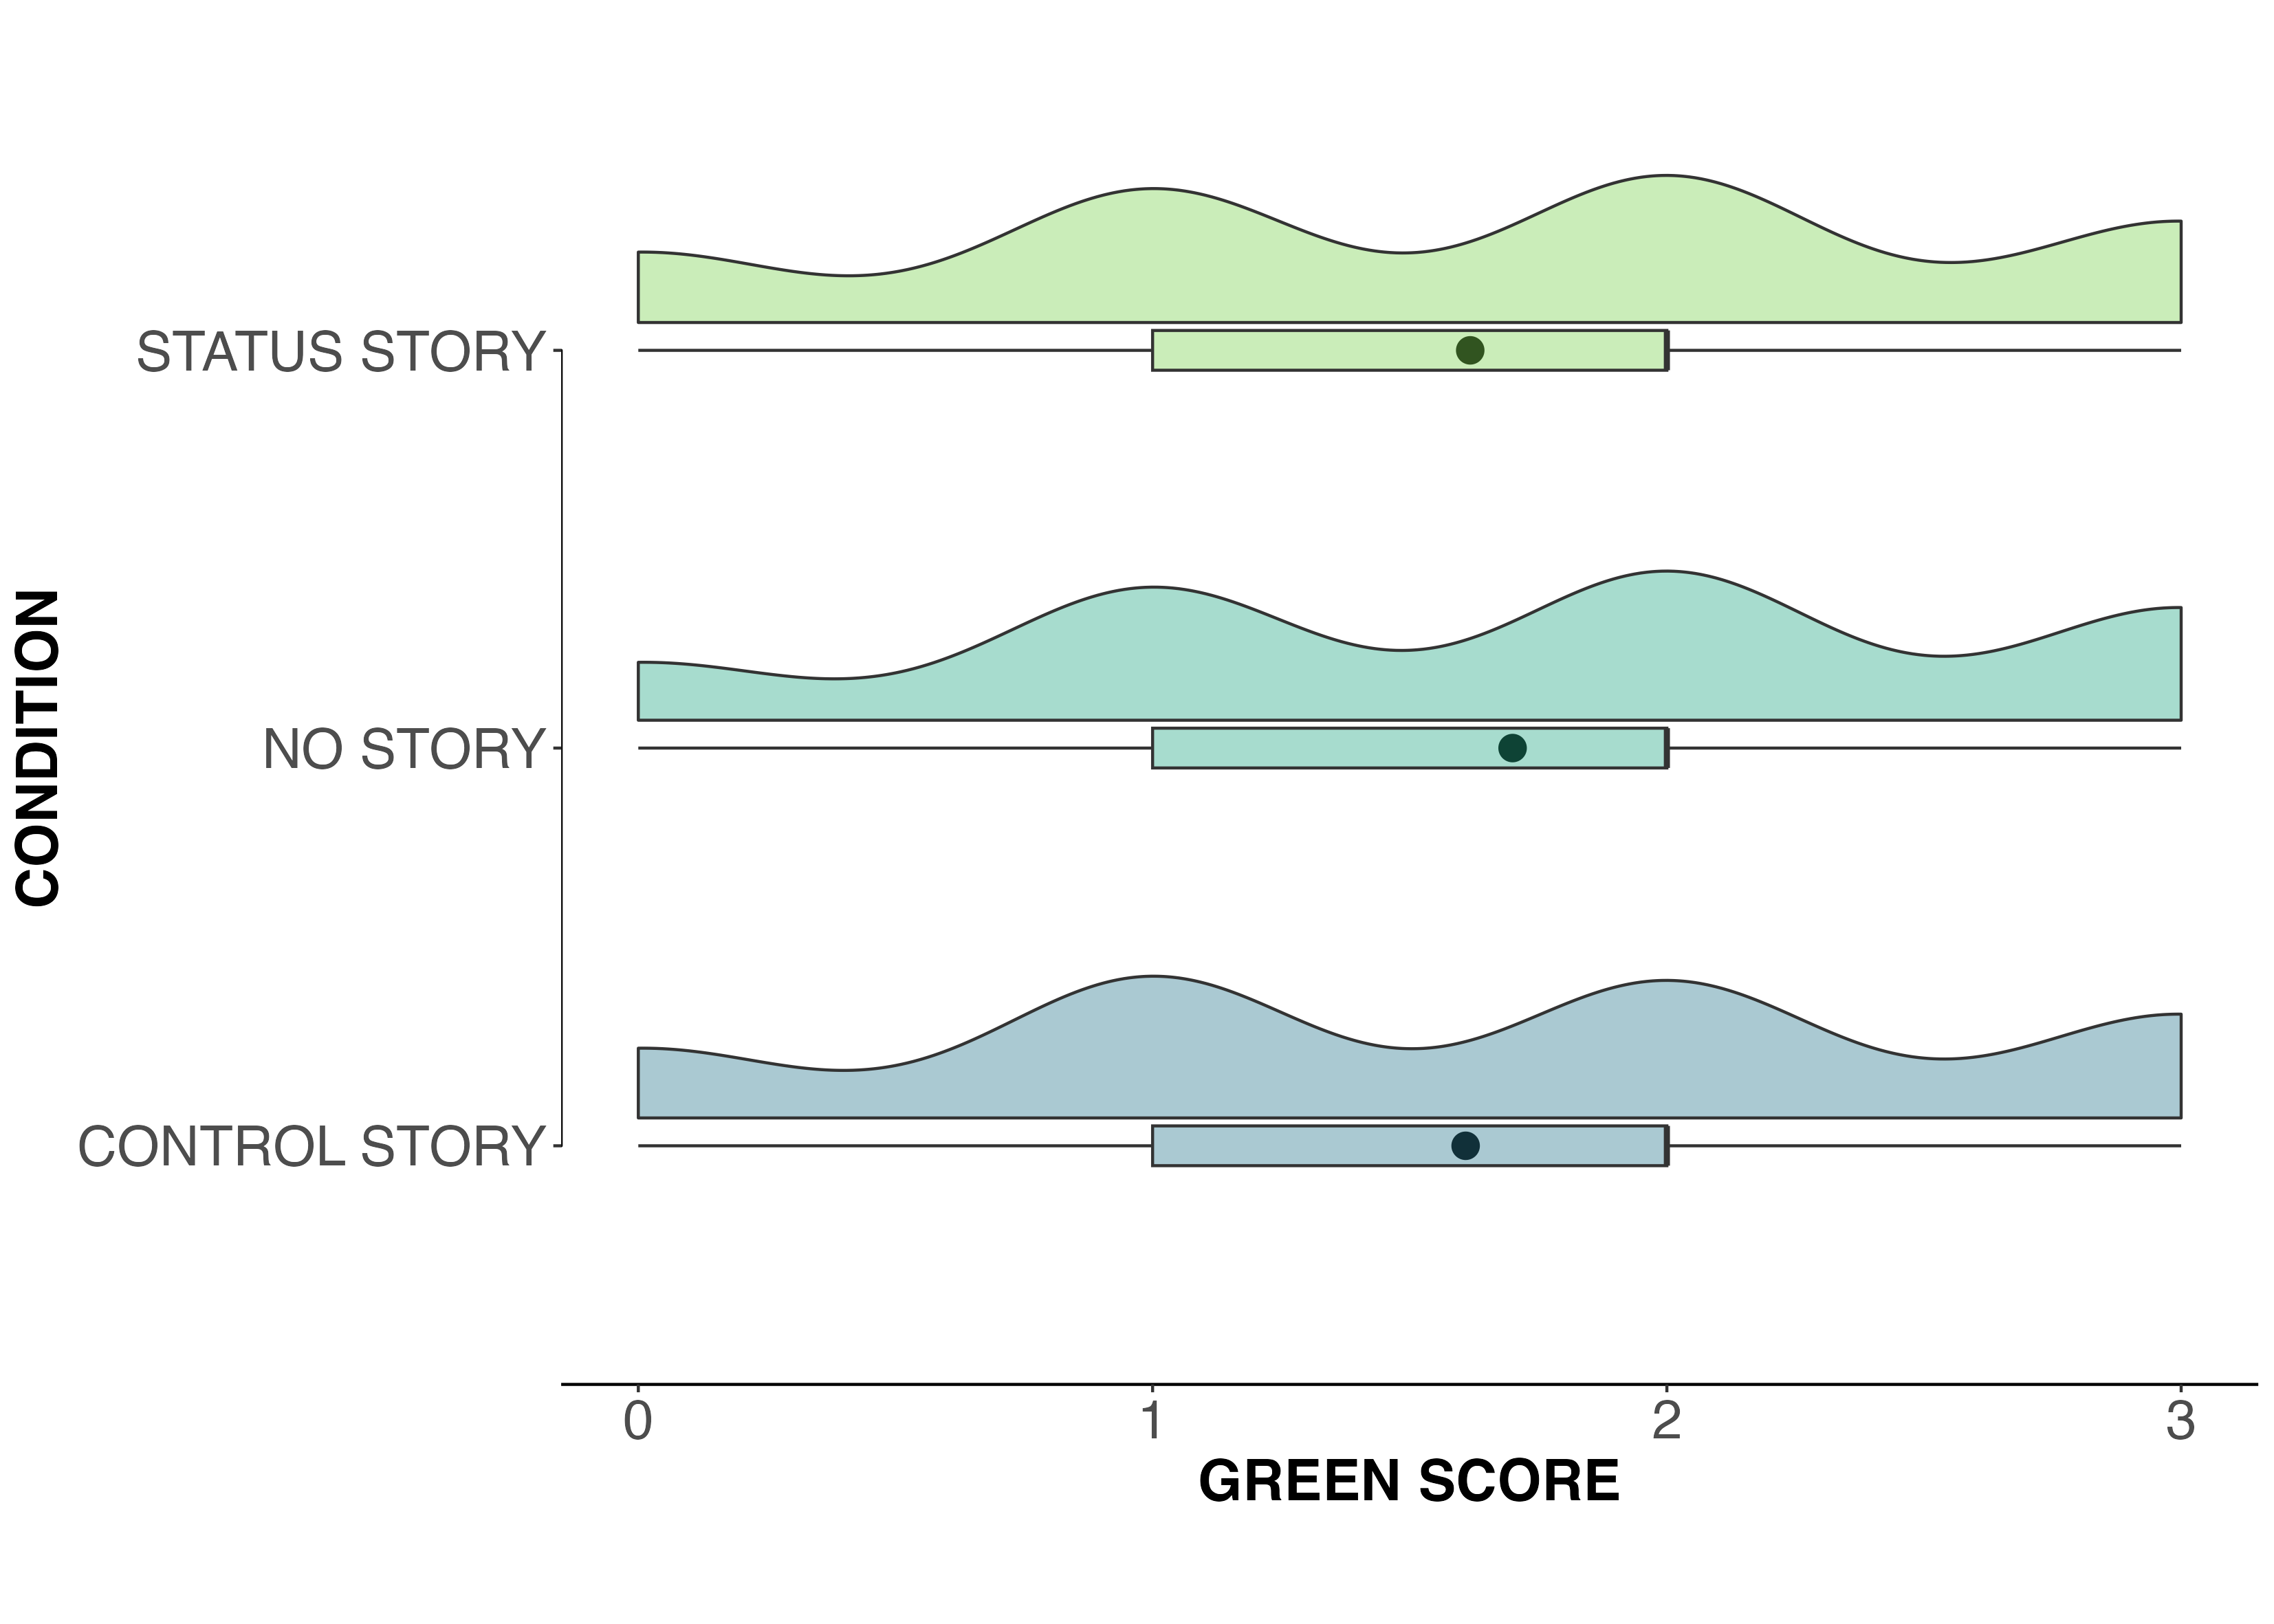
\includegraphics[keepaspectratio]{fig1_updated.png}}
\caption{\textbf{Figure 1}. This diagram shows the distribution of
responses under different conditions. Black dots represent mean values.
Shaded areas below are boxplots corresponding to interquartile ranges.}
\end{figure}

\begin{figure}
\centering
\pandocbounded{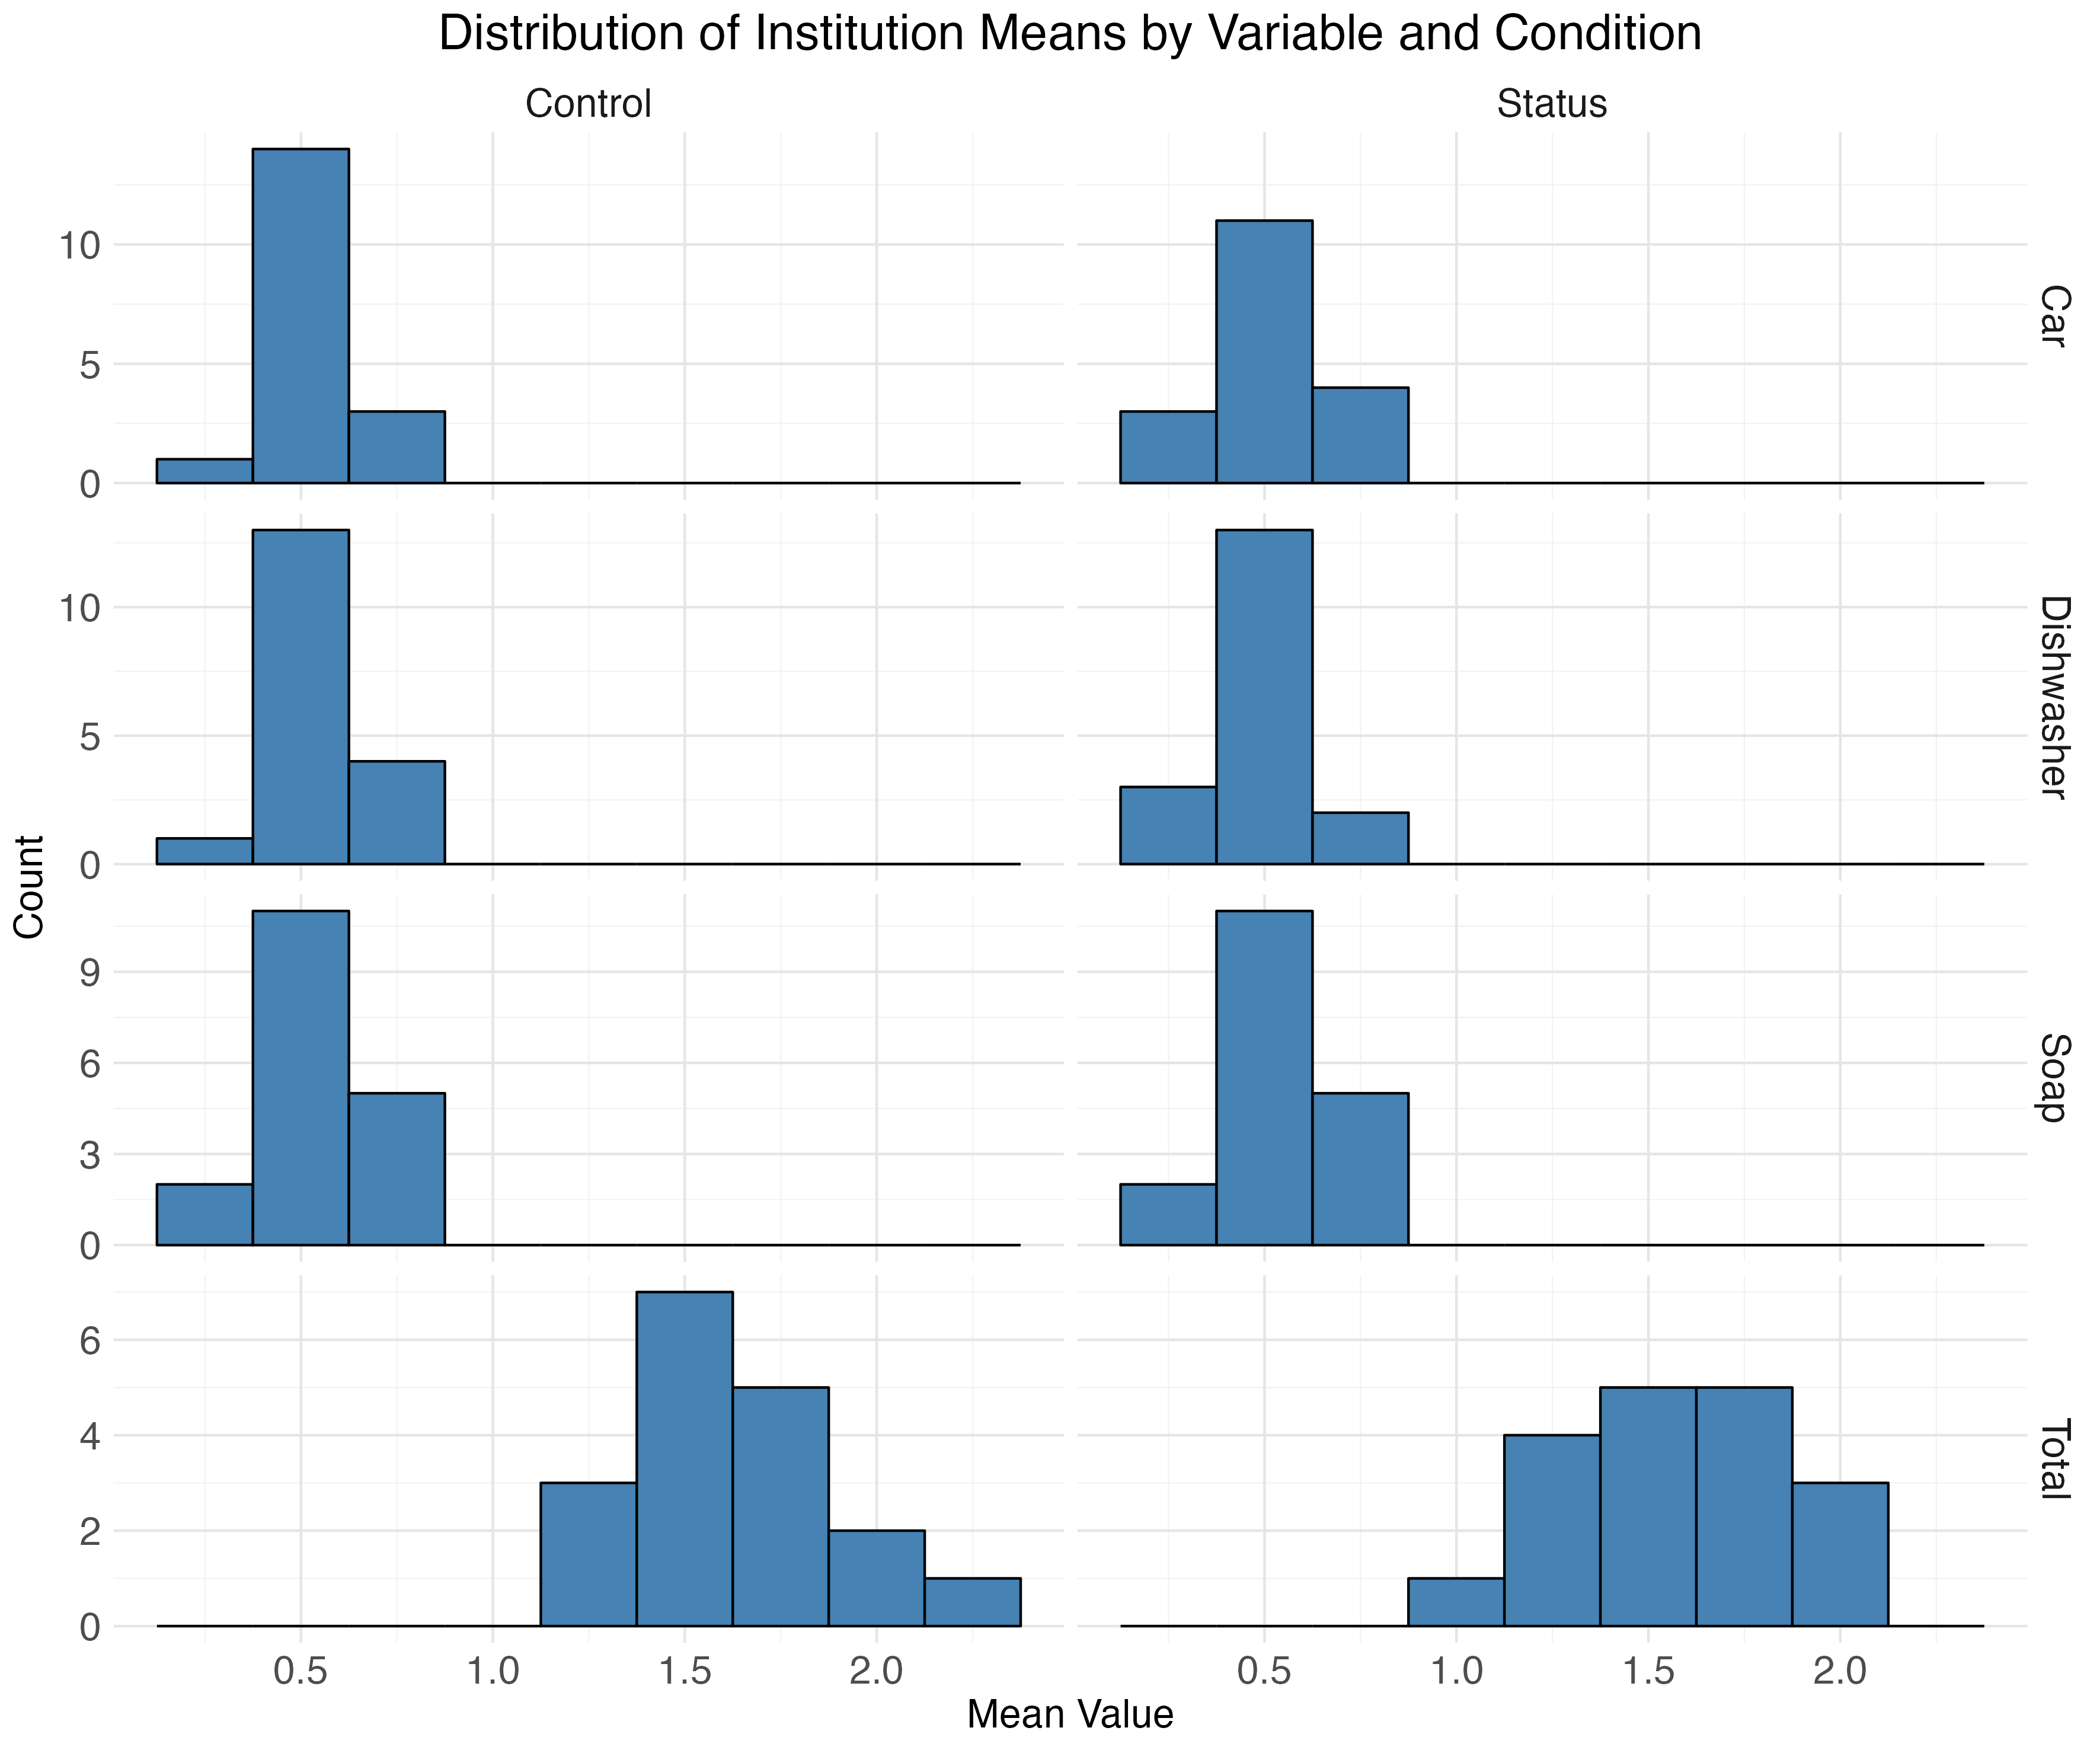
\includegraphics[keepaspectratio]{combined_histograms_clean.png}}
\caption{\textbf{Figure 2}. This diagram shows the distribution of mean
choices for each institution (N = 24) for each product and the composite
score. The means for each product are between 0 and 1 (0 = more
non-green choices by participants, 1 = more green choices), and the mean
for the composite score is between 0 (non-green choices for all three
products) and 3 (green choices for all three products).}
\end{figure}

The original paper by Griskevicius and colleagues (2010) reported a
significant effect of status on the composite score when the status
prime condition was compared to both control conditions (control story
and no story) combined, \emph{F}(1, 166) = 8.53, \emph{p} = .004,
η\textsuperscript{2} = .05, 95\% CI {[}.005, .129{]}. The same test on
our data did not reveal a significant effect, \emph{F}(1, 3,718) = 1.16,
η\textsuperscript{2} \textless{} .001, 95\% CI {[}.000, .002{]}, and in
fact the green score was descriptively lower in the status condition
(\emph{M} = 1.61, \emph{SD} = 1.00) compared to the control condition
(\emph{M} = 1.65, \emph{SD} = 0.99), counter to the original hypothesis.

\subsubsection{Exploratory Analyses}\label{exploratory-analyses}

\paragraph{Prosociality}\label{prosociality}

The original authors made two important notes regarding conditions that
might influence the replicability of the key effect: the prosociality of
``green'' choices and politics. Regarding prosociality, they stressed
that participants' tendency to equate ``green'' choices with prosocial
behavior is fundamental for replication. That is, if participants do not
equate ``green'' choices with prosocial behavior, the effects might be
weakened (resulting in an unsuccessful replication attempt). We are able
to offer a limited response to this issue, as two of our 24 teams added
an extension variable to determine whether participants found owners of
the green products in the study to be more nice, caring, or altruistic
than owners of the non-green products; because these questions were
structured differently across the two sites, we examined each
separately.

The first site (project \#15, \emph{N} = 232) asked participants to
respond to the following question, translated from German: ``Please
indicate on a scale from 1 (disagree completely) to 9 (agree completely)
how much you agree with the following statements: `Consumers of
pro-environmental products are {[}kinder/more empathetic/more
altruistic{]} than consumers of conventional products.'\,'' Here, the
terms ``kind'' and ``more empathetic'' are used as measures of ``nice''
and ``caring,'' respectively. The means for each rating were below the
midpoint of the scale (kind/nice: \emph{M} = 3.58, \emph{SD} = 2.19;
empathetic/caring: \emph{M} = 4.82, \emph{SD} = 2.32; altruistic:
\emph{M} = 4.59, \emph{SD} = 2.17). Importantly, the correlations
between the total composite score (the extent to which people made
``green'' choices) and these characteristic ratings were small and
nonsignificant (kind/nice: \emph{r}(125) = .11, 95\% CI {[}-.07, .28{]},
\emph{p} = .235; empathetic/caring: \emph{r}(125) \textless{} .01, 95\%
CI {[}-.16, .18{]}, \emph{p} = .975; altruistic: \emph{r}(125) = .06,
95\% CI {[}-.12, .23{]}, \emph{p} = .496). Thus, these data do not
provide evidence that perceiving green product choices as altruistic is
associated with choosing green products.

The researchers at this site also included a general question assessing
people's perceptions of the prosociality of green choices. Using the
same rating scale as above, they asked to what extent participants
agreed with this statement (again, translated from German): `Choosing to
buy pro-environmental products is a behavior that is beneficial for the
general public.' Participant ratings for this question were much higher
(\emph{M} = 7.38, \emph{SD} = 1.98) than those for the above questions
about specific characteristics (empathic/caring, reported above),
\emph{t}(126) = 11.03, \emph{p} \textless{} .001, \emph{d} = -0.98, 95\%
CI {[}-1.19, -0.77{]}.

We also tested whether this site's participants' ratings of prosociality
moderated the relationship between condition and composite scores. We
found that participants who rated green choices as more prosocial did
tend to have higher composite scores (\(\beta\) = 0.37, \emph{p}
\textless{} .001), but there was no association between condition and
scores (\(\beta\) = -0.05, \emph{p} = 0.776), and there was no
interaction between condition and ratings of prosociality. In other
words, participants who rated green choices as more prosocial were not
more or less likely to choose those products across the different
conditions (control and status) (\(\beta\) = -0.32), \emph{p} = 0.062).
Summary statistics for this analysis can be found in Table 1.

This site did not replicate the main findings of the original study
(results of a one-way ANOVA comparing composite scores across conditions
{[}status/control{]}: \emph{F}(1, 225) = 0.78, \emph{p} = .378,
η\textsuperscript{2}) = .003, 95\% CI {[}\textless.001, .024{]}. Using
the \emph{pwr} package in \emph{R} (Champely, 2020), we performed a
sensitivity analysis to determine the smallest effect size that could
have been detected with this site's sample size, as well as the sample
size that they would have needed to detect a significant effect (given
the actual effect size that they found). This site had the power to
detect an effect size of η\textsuperscript{2} = .03, and the necessary
sample size to detect a significant effect would have been \emph{n} =
7,843.

The second site (project \#13, \emph{N} = 227) had participants rate the
same three characteristics from 1 (totally agree that the owner has this
quality) to 9 (totally disagree that the owner has this quality). This
group used the same items as had been used by the authors of the
original study to pre-test perceptions of owners of green and non-green
products. We added the ratings of the three green products and the three
non-green products together for each participant and found that
participants rated the owners of green products as nicer (\emph{M} =
9.19, \emph{SD} = 4.21) than owners of non-green products (\emph{M} =
12.19, \emph{SD} = 4.19), \emph{t}(226) = -10.85, \emph{p} \textless{}
.001, \emph{d} = -0.72, 95\% CI {[}-0.87, -0.57{]}. Likewise,
participants rated green product owners as more caring (\emph{M} = 7.95,
\emph{SD} = 3.91) than non-green product owners (\emph{M} = 13.47,
\emph{SD} = 4.32), \emph{t}(225) = -16.35, \emph{p} \textless{} .001,
\emph{d} = -1.09, 95\% CI {[}-1.25, -0.92{]}, and more altruistic
(\emph{M} = 9.83, \emph{SD} = 4.43) than non-green product owners
(\emph{M} = 13.87, \emph{SD} = 4.19) as well, \emph{t}(224) = -10.16,
\emph{p} \textless{} .001, \emph{d} = -0.68 95\% CI {[}-0.82, -0.53{]}.
This site did not replicate the main findings of the original study
(results of a one-way ANOVA comparing composite scores across conditions
{[}status/control{]}: \emph{F}(1, 230) = 0.22, \emph{p} = .639,
η\textsuperscript{2} = .001, 95\% CI {[}\textless.001, .024{]}), despite
having the power to detect an effect size of η\textsuperscript{2} = .03
(the necessary sample size to significantly find the effect that was
actually detected would have been \emph{n} = 2,610.

Therefore, of the two sites that tested whether green consumption was
associated with prosociality, one of them did not find evidence of an
association, and one did find such evidence. Both, however, failed to
replicate the original effect. Thus, it is unlikely that participants'
perceptions of green products as associated with prosociality can
account for whether we did or did not (in actuality, we did not)
replicate Griskevicius and colleagues' (2010) findings. However, we have
to be cautious regarding the conclusions because our results are based
on the very limited number of groups that added these extension
variables.

Next, the original authors regarded political ideology as a relevant
factor in explaining prosocial behavior. Thus, many student teams
included political ideology as extension variables.

\paragraph{Political orientation and party
affiliation}\label{political-orientation-and-party-affiliation}

When the CREP team first contacted the original authors about the
replication, the original authors recommended examining political
orientation as a possible extension variable. A recent meta-analysis by
Cruz (2017) suggested that both political ideology and party affiliation
have associations with environmental concerns. Political orientation
describes where someone falls on the spectrum of political beliefs
ranging from strongly liberal to strongly conservative, and political
party affiliation specifies the major political party with which someone
identifies (Cruz, 2017). However, defining political orientation is
complex, as specific attitudes and beliefs associated with it vary
across time and place (Jost et al., 2003). For example, the
liberal/conservative dimension conveys different political attitudes in
the US versus in European countries (Greenberg \& Jonas, 2003).

In our study, many data collection teams (\emph{N} = 10) added a
question about political orientation (liberal/conservative), and some
(\emph{N} = 4) added a question about political party affiliation
(Republican/Democrat/Independent); some groups added both questions
(\emph{N} = 4), and some groups added similar questions with response
options that were more fitting to their particular country of origin
(e.g., Canada) (more information on characteristics of datasets and
extension variables is available here: \url{https://osf.io/m8uda}). We
used these data to test whether green product selections differed for
liberals and conservatives. Some institutions measured political
orientation with a continuous scale (e.g., from very liberal to very
conservative), whereas others measured it using categorical response
options (e.g., liberal, conservative, neutral). We collapsed over these
different response types to create a novel variable with two levels: a
``liberal'' level that included all responses indicating any degree of
being liberal, and a ``conservative'' level that included all responses
indicating any degree of being conservative. We excluded any ``neutral''
or ``other'' responses. Using this method of collapsing data, we found
that \emph{N} = 551 participants were classified as conservative, while
\emph{N} = 744 participants were classified as liberal. Since this
constitutes just 34.3\% of the overall sample of 3774 participants, it
is unknown whether the effects of political beliefs on status motives,
if detected, would hold for the remaining 65.7\% of participants.
Descriptive statistics for this and all following exploratory analyses
can be found in Table 2.

\subparagraph{Liberal/Conservative}\label{liberalconservative}

We conducted a 2 x 2 factorial ANOVA (political orientation: liberal
vs.~conservative; condition: control vs.~status) to determine whether
political orientation interacted with condition to predict the composite
green score.

We found a main effect of political orientation such that participants
who identified as liberal selected significantly more green products on
average (\emph{M} = 1.87, \emph{SD} = 0.98) than participants who
identified as conservative (\emph{M} = 1.25, \emph{SD} = 0.97),
\emph{F}(1, 1,287) = 130.73, \emph{p} \textless{} .001, η\^{}2 = .092,
95\% CI {[}.064, .124{]}. As we found earlier, there was no main effect
of condition; the mean scores for participants in the grouped control
condition (\emph{M} = 1.65, \emph{SD} = 0.99) did not differ from those
in the status condition (\emph{M} = 1.61, \emph{SD} = 1.00), \emph{F}(1,
1,287) = 0.41, \emph{p} = .522, η\^{}2 \textless{} .001, 95\% CI
{[}\textless.001, .005{]}. There was also no interaction between the two
variables, \emph{F}(1, 1,287) = 0.28, \emph{p} = .597, η\^{}2
\textless{} .001, 95\% CI {[}\textless.001, .005{]}. This analysis had
the power to detect an effect size of η\textsuperscript{2} = .006, and
the necessary sample size to significantly find the effect detected
would have been \emph{n} = 7,845.

\subparagraph{Democrat/Republican}\label{democratrepublican}

Similarly, for political party affiliation (``Democrat'' or
``Republican''), we conducted a 2 x 2 factorial ANOVA (political party:
Democrat \emph{N} = 332 vs.~Republican \emph{N} = 182; condition:
control vs.~status) including only participants from the US.

We found a main effect of political party such that participants who
identified as Democrat selected significantly more green products
(\emph{M} = 1.77, \emph{SD} = 1.03) than participants who identified as
Republican (\emph{M} = 1.12, \emph{SD} = 0.86), \emph{F}(1, 505) =
51.95, \emph{p} \textless.001, η\^{}2 = 0.093, 95\% CI {[}.050, .146{]}.
We detected no main effect of condition (control: \emph{M} = 1.65,
\emph{SD} = 0.99); status: \emph{M} = 1.61, \emph{SD} = 1.00),
\emph{F}(1, 505) = 0.80, \emph{p} = .370, η\^{}2 = .002, 95\% CI
{[}\textless.001, .016{]}), and we did not detect an interaction between
political party and condition, \emph{F}(1, 505) = 0.14, \emph{p} = .709,
η\^{}2 \textless{} .001, 95\% CI {[}\textless.001, .010{]}. This
analysis had the power to detect an effect size of η\textsuperscript{2}
= .015, and the necessary sample size to significantly find the effect
detected would have been \emph{n} = 7,845.

\paragraph{Lab vs.~Online}\label{lab-vs.-online}

To determine whether there were differences in results across different
testing settings, we first collapsed all reported lab settings (group,
individual, and just ``lab'' without specifying whether data were
collected in a group or individually) into one variable level. We then
conducted chi-square tests of independence using a dichotomous setting
variable (lab {[}\emph{N} = 2024{]} versus online {[}\emph{N} =
1581{]}). We found no relationship between green choice and setting for
any of the three types of products (\emph{p}s of .256, .126, and .667
for the green car, soap, and dishwasher, respectively).

To see if there was an interaction between condition and setting, we
conducted a 2 (condition: status vs.~control) x 2 (lab vs.~online) ANOVA
using the composite score as a dependent variable. We did not detect a
mean difference in composite score between those who completed the study
in the lab (\emph{M} = 1.66, \emph{SD} = 0.98) and those who completed
the study online (\emph{M} = 1.64, \emph{SD} = 1.01), \emph{F}(1, 3,547)
= 0.09, \emph{p} = .766, η\^{}2 \textless{} .001, 95\% CI
{[}\textless.001, .001{]}. As we found earlier, there was also no main
effect of condition; the mean scores for participants in the grouped
control condition (\emph{M} = 1.65, \emph{SD} = 0.99) did not differ
from those in the status condition (\emph{M} = 1.61, \emph{SD} = 1.00),
\emph{F}(1, 3547) = 1.27, \emph{p} = .260, η\textsuperscript{2}
\textless{} .001, 95\% CI {[}\textless.001, .003{]}. There was also no
interaction between the two variables, \emph{F}(1, 3,547) = 1.19,
\emph{p} = .275, η\^{}2 \textless{} .001, 95\% CI {[}\textless.001,
.003{]}. This analysis had the power to detect an effect size of
η\textsuperscript{2} = .002, and the necessary sample size to
significantly find the effect detected would have been \emph{n} = 7,845.

\paragraph{US vs.~others}\label{us-vs.-others}

The original study was conducted only with individuals in the United
States. Here, we conducted an exploratory analysis to determine whether
the tested effects differed for US-based participants versus
participants from other countries. Using data from US-based participants
only (\emph{N} = 2,151), we found no association between condition
(control versus status) and green car selection (𝛘\textsuperscript{2}(1,
\emph{N} = 2,104)) = 0.12, \emph{p} = .728, ɸ = 0.01, 95\% CI
{[}\textless.001, .053{]}), green cleaner selection
(𝛘\textsuperscript{2}(1, N = 2,103)) = 0.004, \emph{p} = .884, ɸ =
0.001, 95\% CI {[}\textless.001, .034{]}), or green dishwasher
(𝛘\textsuperscript{2}(1, N = 2,107)) = 0.000, \emph{p} = .952, ɸ
\textless.001, 95\% CI {[}\textless.001, .022{]}) selection.

We then conducted a 2 x 2 ANOVA to test whether there was a main effect
of condition (control or status) or interaction with geographic setting
(US or non-US). We detected no significant main effect of condition
(\emph{p} = .558) or interaction (\emph{p} = .409). We found a small
main effect of location, such that individuals from non-US countries
selected significantly more green products (\emph{M} = 1.83, \emph{SD} =
0.95) than individuals from the US (\emph{M} = 1.48, \emph{SD} = 1.01),
\emph{F}(1, 3,714) = 115.62, \emph{p} \textless{} .001,
η\textsuperscript{2} = .030, 95\% CI {[}.020, .042{]}. This analysis had
the power to detect an effect size (for the interaction) of
η\textsuperscript{2} = .002, and the necessary sample size to
significantly find the effect detected would have been \emph{n} = 7,845.

\paragraph{Stability of effect over
time.}\label{stability-of-effect-over-time.}

To determine whether any effects differed over the time period in which
we collected data, we examined effects across projects that were started
in different years, as determined by their project codes assigned at the
time the teams signed up for the study (e.g., project \#14-3 was
initiated in 2014). With year treated as a factor, we examined whether
there were any differences in composite green scores across conditions
(control and status). As demonstrated in Figure 3, we did not detect any
meaningful change in effect size over time. If we used a linear
regression model to predict effect size by year, we would need 7,843
teams to detect an effect of η\textsuperscript{2} = .001, and the
analysis with \emph{n} = 24 teams had the power to detect an effect of
η\textsuperscript{2} = .26.

\begin{figure}
\centering
\pandocbounded{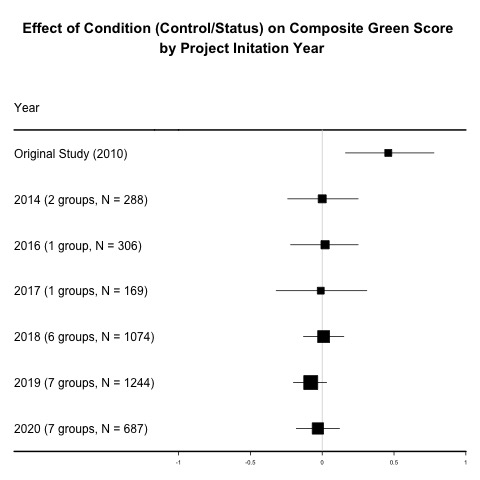
\includegraphics[keepaspectratio]{forestplot.jpg}}
\caption{\textbf{Figure 3.} Effect sizes (Cohen's d) by year with 95\%
confidence intervals.}
\end{figure}

\paragraph{Gender differences}\label{gender-differences}

In their original paper, Griskevicius and colleagues (2010) stated that
exploring gender differences would be interesting in future studies.
Although they did not find any gender differences, Griskevicius et
al.~(2010) hypothesized that men could be more likely to engage in
pro-environmental ``showing-off'' behavior than women because men are
generally more concerned about status motives. Because of the increased
statistical power that our large sample provided, we sought to test
these potential gender differences as part of our exploratory analyses.

To test this question, we conducted a 2 x 2 factorial ANOVA (gender:
woman or man; condition: control vs.~status). We found a main effect of
gender, such that participants who identified as women selected
significantly more green products (\emph{M} = 1.69, \emph{SD} = 0.99)
than participants who identified as men (\emph{M} = 1.46, \emph{SD} =
1.01), \emph{F}(1, 3,263) = 36.22, \emph{p} \textless{} .001, η\^{}2 =
0.010, 95\% CI {[}.005, .019{]}. We did not detect an interaction
between gender and condition, \emph{F}(1, 3,263) = 0.00, \emph{p} =
.964, η\textsuperscript{2} \textless{} .001, 95\% CI {[}\textless.001,
\textless.001{]}. This analysis had the power to detect an effect size
(for the interaction) of η\textsuperscript{2} = .002, and the necessary
sample size to significantly find the effect detected would have been
\emph{n} = 7,845.

When we conducted a 2 x 3 factorial ANOVA with the independent
conditions (control, status, and no story), we found an effect of
condition, \emph{F}(2, 3,261) = 4.23, \emph{p} = .015, η\^{}2 = .001,
η\textsuperscript{2} = .010, 95\% CI {[}\textless.001, .005{]}. Post-hoc
testing with Tukey's HSD correction revealed significant differences
between the ``no story'' condition and the other two conditions (95\% CI
of the difference for no story vs.~control story: {[}0.01, 0.21{]},
\emph{p} = .028; 95\% CI of the difference for no story vs.~status:
{[}-0.21, -0.01{]}, \emph{p} = .032). There was no difference between
the control story and the status story conditions, \emph{p} = .995.
Participants in the ``no story'' condition made more ``green'' choices
(\emph{M} = 1.7, \emph{SD} = 0.98) than participants in the control
condition (\emph{M} = 1.58, \emph{SD} = 1.01) or status condition
(\emph{M} = 1.59, \emph{SD} = 1.00). This effect was not detected when
the ungrouped conditions were examined in the entire data set; it was
detected only when we excluded participants who did not respond to the
question about gender or listed a gender other than ``Male'' or
``Female.''

\subsubsection{Internal meta-analysis}\label{internal-meta-analysis}

To synthesize data collected in all groups, and investigate whether the
tested effects varied across data collection sites, we performed a
random effects internal meta-analysis for the overall model with no
moderators and then separately for each moderator included in the model.
The results from these analyses corroborated the analyses reported
above: None of the tested effects were significant (see Table 3). The
same was true for all of the moderating effects of extension variables.

\subsection{Discussion}\label{discussion}

In their original study, Griskevicius et al.~(2010) suggested that
hypothetical pro-environmental behavior can be promoted by priming
status motives. They linked this finding to the ``competitive altruism''
hypothesis, according to which individuals' altruistic behaviors arise
from status competition (i.e., attempts to be perceived as good; Hardy
\& Van Vugt, 2006). In essence, cultivating a positive reputation
through prosocial and pro-environmental behavior and action, coupled
with a demonstrated willingness to incur costs for the public good, can
elevate an individual's standing within a group. The original study
revealed a higher preference for all three hypothetical green products
(green car, green cleaner, green dishwasher) in the status condition
compared to the control conditions.

In this multi-lab replication study, we recruited a large sample of
participants across six different countries. We employed the same
methods and analytical strategy as the original study. As part of our
pre-registered confirmatory analysis, we tested whether an effect of
reading the status story on pro-environmental choice behavior existed
when the green score was calculated as a composite. Critically, this
analysis did not detect a statistically significant effect of the status
story, failing to replicate the original findings from Experiment 1 of
Griskevicius et al.~(2010). We also analyzed whether an effect of
reading the status story existed for each of the green vs.~non-green
products separately. For all three products, we failed to detect a
significant effect of the status story. Participants in the status
condition and the control conditions did not differ in their tendency to
select hypothetical green products. As in the original study, we found
no differences in green choice behavior between the two control
conditions (non-status story vs.~no story). Thus, overall, we did not
replicate the main conclusion of Experiment 1 from Griskevicius et
al.~(2010) with a much more highly powered analysis (original \emph{N} =
168, present \emph{N} = 3774).

There are several possible explanations for this difference in results.
The most straightforward is simply that the original study was a false
positive, and there was no true effect of priming status motives. The
literature reports on the ``going green to be seen'' effect has reported
varied results across replication attempts (see Brick et al., 2017;
Brick \& Sherman, 2021; Lange et al., 2020). In an effort to clarify
these varied results, our results fail to provide evidence that
pro-environmental behavior is driven by status motives.

Another explanation for the present null results might lie in the
decision to use the same priming technique as Griskevicius and
colleagues (2010) to induce status motives. The literature in this area
examining pro-environmental behavior has produced a variety of findings,
depending on the method used. Some studies have demonstrated that
reputational cues can increase pro-environmental behavior, particularly
when behavior is observable or occurs in public contexts. For example,
public goods games and reputation-based interventions have shown that
when individuals can gain social standing from their choices,
pro-environmental behavior tends to increase (Barclay \& Barker, 2020;
Milinski et al., 2006). Similarly, recent work has shown that priming
the future or evoking social comparison can activate status concerns and
promote sustainable choices (Essl et al., 2024). In contrast, other
studies using priming or visibility manipulations have failed to find
such effects (Brick \& Sherman, 2021; Lange et al., 2020; Henkel et al.,
2019). While these studies are not direct replications of Griskevicius
et al.~(2010), they test closely related theoretical claims. Therefore,
these competing results warrant further investigation into the
appropriateness of the variety of methods that have been used to study
pro-environmental behavior.

One more explanation for our null results hinges on the finding that our
control participants selected the green products at much higher rates
than in the original study. Our control participants' rates of selecting
the green car, soap, and dishwasher were 55.5\%, 56.8\%, and 52.9\%,
respectively, while the original control participants' rates were much
lower at 37.2\%, 25.7\%, and 34.5\%, respectively. Green products may
have been perceived as more novel when Griskevicius and colleagues ran
their study (\textasciitilde2008) relative to when we ran ours
(2014-2020), so that a smaller group of the population would buy them
when given the choice. In this case, perhaps status primes moved some
people's preferences from that low baseline. On the other hand, perhaps
by the time our data collection occurred, the people who could have been
persuaded by a status prime to buy green products were already making
these choices because of those products' popularity in broader culture.

Given this possible alternative explanation, we examined whether there
appeared to be any overall pattern in the total composite score over
time (collapsing across conditions). Extended duration of data
collection, spanning several years, allowed us to investigate potential
variations in the tested effects over time. As shown in Figure 4, the
scores documented in some years did differ from others, but the early
years (2014 and 2016) did not yield significantly different scores from
the last two years (2019 and 2020). Nevertheless, it is still possible
that attitudes toward pro-environmental behaviors had sufficiently
changed between the time when Griskevicius et al.~(2010) conducted their
study (which appeared to have occurred in 2008 or earlier, based on the
date of original submission to the \emph{Journal of Personality and
Social Psychology}) and 2014, the earliest starting date of data
collection in our study.

\begin{figure}
\centering
\pandocbounded{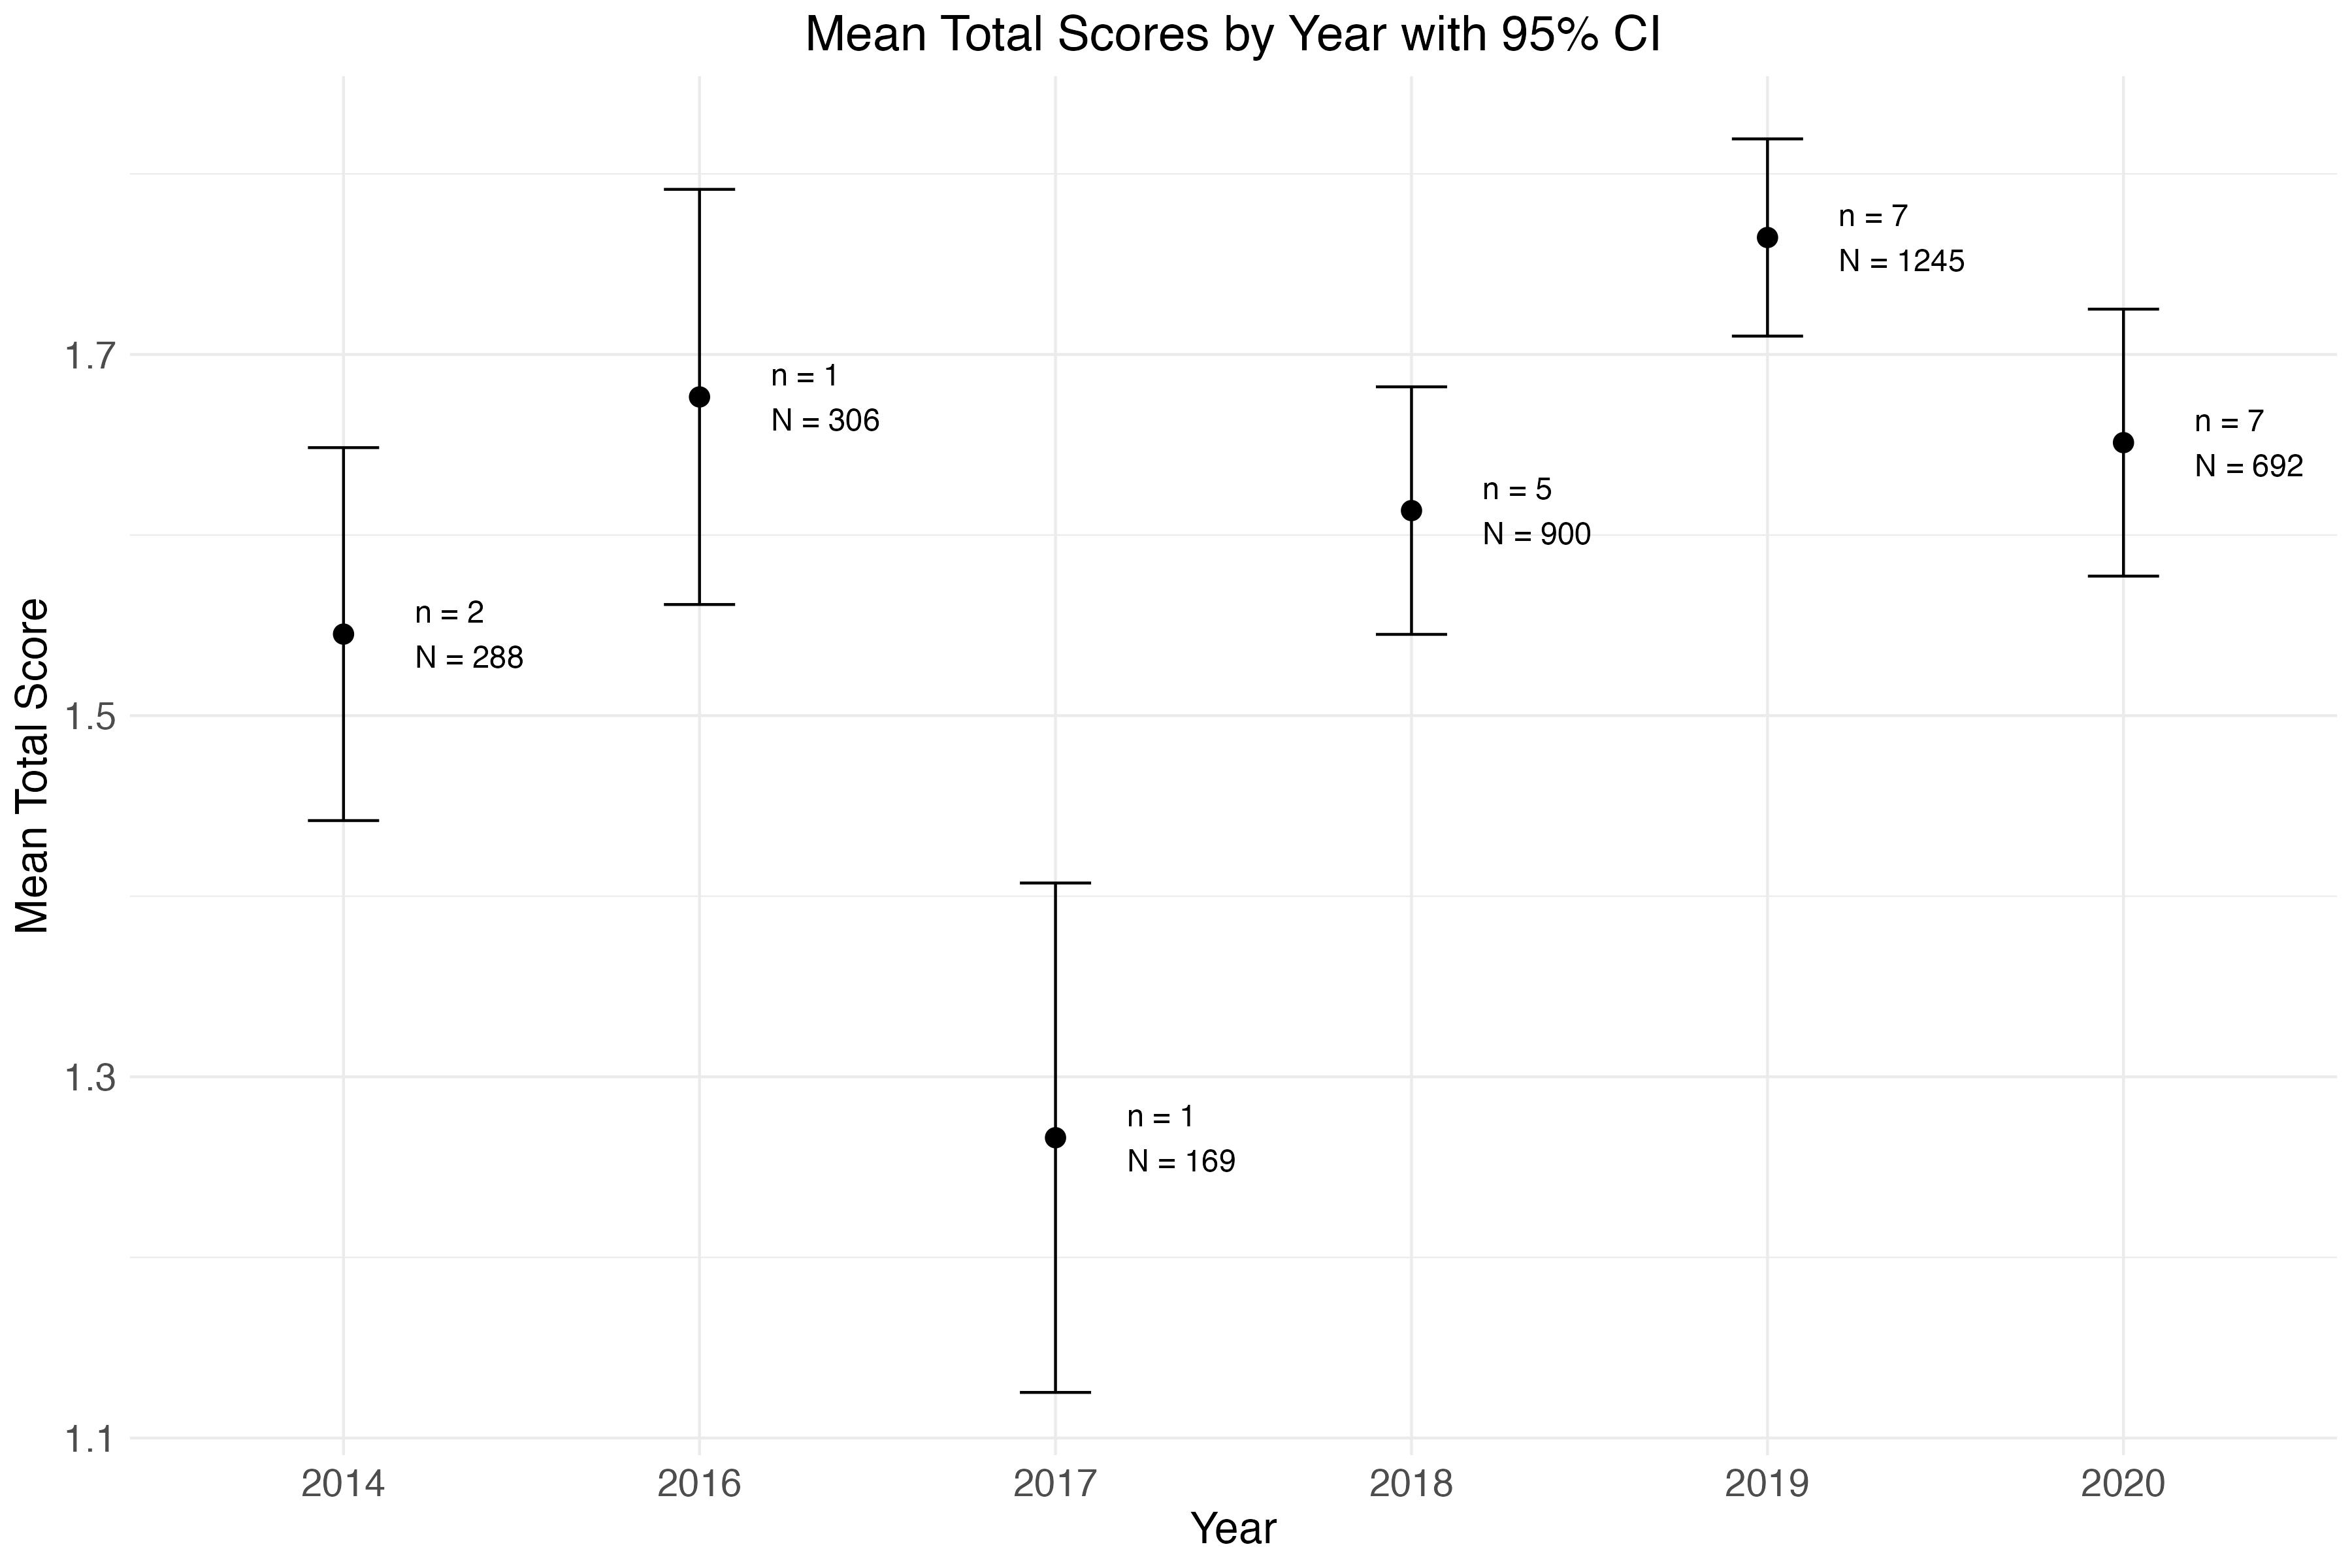
\includegraphics[keepaspectratio]{fig4.jpg}}
\caption{\textbf{Figure 4.} Mean composite scores by year. There were no
noticeable differences in mean composite scores between the earliest
projects (2014 and 2015) and the latest projects (2019 and 2020). n =
Number of projects, N = total sample size.}
\end{figure}

The original authors stressed that to document an effect of status
motives on pro-environmental choices, it is essential that participants
equate these choices with prosocial behavior. Despite being recommended
by the original authors, only two groups decided to explore this issue
directly, and their findings suggested that whether participants thought
of pro-environmental choices in this way was unrelated to those
participants' responses. Thus, although the original authors' claim was
only tested in a limited subset of our sample, we have not found support
for it.

Per the recommendation of the original authors, we also performed
exploratory analyses to test whether political beliefs significantly
moderated the effect of reading the status story on pro-environmental
choices. In this study, some testing sites collected data on political
orientation (e.g., liberal/conservative) and/or political party (e.g.,
Democrat/Republican) as extension variables. We found that participants
who identified as liberal or as Democrats selected more green products
than participants who identified as conservatives or as Republicans.
These independent effects of political belief (either orientation or
party affiliation) did not, however, interact with any effect of reading
the status story on green choice behavior. Although pro-environmental
behavior is typically associated with left-wing orientation (at least in
the United States), Barclay and Barker (2020) offered an alternative
explanation. Namely, they suggest that people of more conservative
ideologies might also regard pro-environmental behavior highly, because
according to their model, behind it lies cooperative reputation.

One difference between the original study and our multi-site replication
was that in the original study, participants were tested in small groups
in a lab setting. Meanwhile, in our study, many sites tested
participants in the lab, sometimes individually and sometimes in small
groups, yet other sites tested participants online. It is conceivable
that being tested in a laboratory context, which is presumably more
social (in that, at minimum, the participant has some interaction with a
research assistant, and possibly with other participants), may more
strongly influence status motives on pro-environmental behaviors,
compared to being tested online. If this is the case, then we would
expect to have found differences in the proportion of green choice
selections between in-person and online participants in our study (e.g.,
Belletier et al., 2015; Belletier \& Camos, 2018). However, we found no
significant difference in composite green scores across these settings
when we explored whether the setting in which participants were tested
(lab---presumably at least somewhat social---versus online) influenced
the results. Thus, we cannot conclude that the difference between the
present study and that of the original study can be explained by
different testing environments. Online data collection has become
increasingly popular over the last decade and offers several advantages
over traditional lab settings, such as reduced costs, more effective
testing, increased generalizability of results, and more efficient
(i.e., automated) data collection (e.g., Buhrmester et al., 2011;
Dandurand et al., 2008; Gosling et al., 2004; Nayak \& Narayan, 2019).
Our findings -- that there were no differences in results between the
lab and online contexts -- are consistent with those of many previous
studies comparing the quality of online and lab-based samples of
participants (e.g., Peer et al., 2017; Riva et al., 2003).

It is important to note that the original study was conducted in the US,
while this multi-site replication project collected data in five other
countries: Canada, the Netherlands, the UK, Germany, and Iceland. We
found no significant differences in results between the samples from
different countries. This is not surprising given that all of the
countries included here are WEIRD (Western, Educated, Industrialized,
Rich, and Democratic; Henrich et al., 2010), with similar environmental
policies according to the Fragile State Index (Fund for Peace, 2022).
Whether the relation between status motives and pro-environmental
behaviors differs in non-WEIRD populations is an important area for
future work.

Finally, in their paper, Griskevicius and associates stated that gender
differences in status motives would be worth exploring. Our findings
indicate a greater preference for green products among women compared to
men, but a moderating effect of gender on the relationship between the
experimental conditions and product preference was not detected.

All of the results that we documented with our pooled data were
corroborated by the internal meta-analysis that we performed. The
primary effect and any moderating effects of extension variables were
all non-significant, and did not vary across the different testing
sites. Taken together, these findings fail to suggest that
pro-environmental behavior can be promoted by priming status motives, at
least using the present priming paradigm.

\subsubsection{Limitations of the study}\label{limitations-of-the-study}

The present study has some limitations. First, as noted above, all of
the countries in which the study was conducted are WEIRD and have
similar environmental policies. Thus, we urge caution in generalizing
these findings to other populations. One possibility is that
participants from non-WEIRD and fragile countries, many of which have
recently increased efforts to promote pro-environmental behaviors (e.g.,
Díaz et al., 2020), could be more sensitive to any potential relation
between social status and pro-environmental action. Therefore, it will
be worth exploring in future work whether the results of the original
study replicate in non-WEIRD environments and countries that are
considered fragile. Additionally, it is crucial to acknowledge the
potential impact of socio-cultural factors in these diverse contexts.
Pro-environmental behavior is influenced by social norms (e.g.,
Saracevic et al., 2022) and individual values (e.g., Nordlund \&
Garvill, 2002). Thus, we recommend that future researchers explore how
local values and socio-economic conditions might influence the
relationship between social status and pro-environmental actions in
different regions.

Second, we tested moderation effects only for those variables for which
we had sufficient statistical power. Therefore, most of the extension
variables that were measured could not be used in the analyses (e.g.,
personality traits, altruism, empathy). To more thoroughly explore the
role of extension variables in the effects being replicated, future CREP
studies could pose stricter guidelines on the usage of extension
variables in student groups. Furthermore, incorporating a comprehensive
set of guidelines for the inclusion of extension variables would enhance
the robustness and applicability of findings across diverse research
settings, fostering a more nuanced understanding of moderation effects.

Third, there is a possibility that the minimal priming manipulation did
not effectively induce status motives. The original Griskevicius et
al.~(2010) study did not include a manipulation check, instead
referencing earlier work (Griskevicius et al., 2009) in which the
manipulation produced very large effects on self-reported desire for
status (e.g., d = 3.78). Following the CREP protocol, our replication
sites were not required to include a manipulation check. However, one
team did include such a check and found that while the manipulation had
a statistically detectable effect, the effect size was substantially
smaller than that reported in the original study (d = 0.32 vs.~d = 3.78
for the composite measure), suggesting that the manipulation was not as
psychologically potent in the replication. At the same time, there are
reasons to be cautious about interpreting the original effect sizes,
which are higher than the 99th percentile of all effects observed within
social psychology (Lovakov \& Agadullina, 2021). This reported effect is
unusually large, arising from reading a paragraph, and is dependent on
control group means that suggest an implausibly low baseline desire for
status. Together, the results of 24 replications suggest that this
paragraph does not cause changes in choosing to purchase a green product
in the same manner as originally reported in Griskevicius et al., 2010,
but it is unclear to what extent the null results reflect a failure of
the original manipulation or a challenge to the underlying theory.

\subsubsection{Conclusion}\label{conclusion}

One goal for this project was to provide a medium for students to engage
in high-quality replication research while contributing to psychological
science. Student-led projects can and do offer rigorous experience, and
the present work is no exception; the quality of the studies was ensured
by continuous and careful supervision of senior researchers (faculty
members, two reviewers, one CREP board member), recommendations from the
original first author, and documentation of the research process (e.g.,
Grahe et al., 2020; Wagge, Brandt, et al., 2019, Wagge, Hurst, et al.,
2023).

The primary goal of this project, however, was to investigate the
possibility that pro-environmental behavior can be promoted by priming
status motivations. This study presents a large sample, multi-site
replication of the Griskevicius et al.~(2010) study, conducted by
student teams at various institutions. Overall, our study did not
replicate the original work, as we observed no evidence supporting the
notion that hypothetical pro-environmental behavior can be stimulated by
reading a story designed to prime status motives. While these results do
not dismiss the theoretical framework proposed by Griskevicius et al.,
they do, at the very least, indicate that there are substantial boundary
conditions for the expected effect. Given our inability to demonstrate a
reliable effect, proponents of the original theory should reconsider
which populations may still exhibit an effect using the present methods,
as well as potential explanations for why the effect may have diminished
in the intervening years. The time lapse between the original study and
our replications, spanning from 4 to 10 years, has seen increased
attention directed toward climate change and environmental choices in
many communities. It is conceivable that the heightened awareness of
this topic in the general population has tempered the likelihood of the
effect to emerge. Regardless of cause, it seems the original effect is
either very sensitive to the conditions in which it is tested, or cannot
be reliably detected in modern times.

\newpage

\subsection{References}\label{references}

Arnold, J. B. (2019). ggthemes: Extra Themes, Scales and Geoms for
`ggplot2'. R package version 4.2.0.
\url{https://CRAN.R-project.org/package=ggthemes}

Aust, F., \& Barth, M. (2024). \emph{papaja: Prepare reproducible APA
journal articles with R Markdown}.
\url{doi:10.32614/CRAN.package.papaja}, R package version 0.1.3,
\url{https://github.com/crsh/papaja}.

Barclay, P., \& Barker, J. L. (2020). Greener than thou: people who
protect the environment are more cooperative, compete to be
environmental, and benefit from reputation. \emph{Journal of
Environmental Psychology}, 72, 101441.
\url{https://doi.org/10.1016/j.jenvp.2020.101441}

Belletier, C., \& Camos, V. (2018). Does the experimenter presence
affect working memory? \emph{Annals of the New York Academy of Sciences,
1424,} 212--220. \url{https://doi.org/10.1111/nyas.13627}

Belletier, C., Davranche, K., Tellier, I. S., Dumas, F., Vidal, F.,
Hasbroucq, T., \& Huguet, P. (2015). Choking under monitoring pressure:
Being watched by the experimenter reduces executive attention.
\emph{Psychonomic Bulletin \& Review, 22,} 1410--1416.
\url{https://doi.org/10.3758/s13423-015-0804-9}

Bonett, D. (2024). statpsych: Statistical Methods for Psychologists. R
package version 1.6.0,
\url{https://CRAN.R-project.org/package=statpsych}.

Braun Kohlová, M., \& Urban, J. (2020). Buy green, gain prestige and
social status. \emph{Journal of Environmental Psychology}, 69, 101416.
\url{https://doi.org/10.1016/j.jenvp.2020.101416}

Brick, C., Sherman, D. K., \& Kim, H. S. (2017). ``Green to be seen''
and ``brown to keep down'': Visibility moderates the effect of identity
on pro-environmental behavior. \emph{Journal of Environmental
Psychology}, 51, 226-238.
\url{https://doi.org/10.1016/j.jenvp.2017.04.004}

Brick, C., \& Sherman, D. K. (2021). When does being watched change
pro-environmental behaviors in the laboratory?. \emph{Sustainability},
13(5), 2766. \url{https://doi.org/10.3390/su13052766}

Buchanan, E., Gillenwaters, A., Scofield, J., \& Valentine, K (2019).
\emph{MOTE: Measure of the Effect: Package to assist in effect size
calculations and their confidence intervals}. R package version 1.0.2,
\url{http://github.com/doomlab/MOTE}.

Buhrmester, M., Kwang, T., \& Gosling, S. D. (2011). Amazon's Mechanical
Turk: A new source of inexpensive, yet high-quality, data?
\emph{Perspectives on Psychological Science, 6}(1), 3--5.
\url{https://doi.org/10.1177/1745691610393980}

Champely, S. (2020). \emph{pwr: Basic Functions for Power Analysis}. R
package version 1.3-0, \url{https://github.com/heliosdrm/pwr}.

Cruz, S. M. (2017). The relationships of political ideology and party
affiliation with environmental concern: A meta-analysis. \emph{Journal
of Environmental Psychology, 53,} 81-91.
\url{https://doi.org/10.1016/j.jenvp.2017.06.010}

Dandurand, F., Shultz, T. R., \& Onishi, K. H. (2008). Comparing online
and lab methods in a problem-solving experiment. \emph{Behavior Research
Methods, 40}(2), 428--434. \url{https://doi.org/10.3758/BRM.40.2.428}

Díaz, M. F., Charry, A., Sellitti, S., Ruzzante, M., Enciso, K., \&
Burkart, S. (2020). Psychological factors influencing pro-environmental
behavior in developing countries: Evidence from Colombian and Nicaraguan
students. \emph{Frontiers in Psychology, 11,} 580730.
\url{https://doi.org/10.3389/fpsyg.2020.580730}

Eurobarometer (2017). Attitudes of European citizens towards the
environment. Retrieved from
\url{https://data.europa.eu/euodp/data/dataset/S2156_88_1_468_ENG}

Essl, A., Hauser, D., \& von Bieberstein, F. (2024). Let's think about
the future: The effect of positive and negative future primes on
pro-environmental behavior. \emph{Journal of Behavioral and Experimental
Economics}, 109, 102166.
\url{https://doi.org/10.1016/j.socec.2024.102166}

Frank, M. C., \& Saxe, R. (2012). Teaching Replication.
\emph{Perspectives on Psychological Science, 7}(6), 600--604.
\url{https://doi.org/10.1177/1745691612460686}

Fund for Peace (2022). Fragile State Index 2022 - Annual Report.
Retrieved from
\url{https://fragilestatesindex.org/2022/07/13/fragile-states-index-2022-annual-report/}

Garnier, S., Ross, N., Rudis, R., Camargo, P. A., Sciaini, M., \&
Scherer, C. (2024). \emph{viridis(Lite) - Colorblind-Friendly Color Maps
for R}. \url{doi:10.5281/zenodo.4679423}, viridis package version 0.6.5,
\url{https://sjmgarnier.github.io/viridis/}.

Ghelfi, E., Christopherson, C. D., Urry, H. L., Lenne, R. L., Legate,
N., Ann Fischer, M., Wagemans, F. M. A., Wiggins, B., Barrett, T.,
Bornstein, M., de Haan, B., Guberman, J., Issa, N., Kim, J., Na, E.,
O'Brien, J., Paulk, A., Peck, T., Sashihara, M., \ldots{} Sullivan, D.
(2020). Reexamining the effect of gustatory disgust on moral judgment: A
multilab direct replication of Eskine, Kacinik, and Prinz (2011).
\emph{Advances in Methods and Practices in Psychological Science, 3}(1),
3--23. \url{https://doi.org/10.1177/2515245919881152}

Goldstein, N. J., Cialdini, R. B., \& Griskevicius, V. (2008). A room
with a viewpoint: Using social norms to motivate environmental
conservation in hotels. \emph{Journal of Consumer Research}, 35(3),
472-482. \url{https://doi.org/10.1086/586910}

Gordon. M., \& Lumley, T. (2024). \emph{forestplot: Advanced Forest Plot
Using `grid' Graphics}. R package version 3.1.6,
\url{https://github.com/gforge/forestplot}.

Gosling, S. D., Vazire, S., Srivastava, S., \& John, O. P. (2004).
Should We Trust Web-Based Studies? A Comparative Analysis of Six
Preconceptions About Internet Questionnaires. \emph{American
Psychologist, 59}(2), 93--104.
\url{https://doi.org/10.1037/0003-066X.59.2.93}

Grahe, J. E. (2017). Authentic research projects benefit students, their
instructors, and science. In How we teach now: The GSTA guide to
student-centered teaching. (pp.~352--368). Society for the Teaching of
Psychology. Retrieved from
\url{https://teachpsych.org/ebooks/howweteachnow}

Grahe, J. E., Cuccolo, K., Leighton, D. C., \& Cramblet Alvarez, L. D.
(2020). Open science promotes diverse, just, and sustainable research
and educational outcomes. \emph{Psychology Learning \& Teaching, 19}(1),
5--20. \url{https://doi.org/10.1177/1475725719869164}

Grahe, J. E., Reifman, A., Hermann, A. D., Walker, M., Oleson, K. C.,
Nario-Redmond, M., \& Wiebe, R. P. (2012). Harnessing the undiscovered
resource of student research projects. \emph{Perspectives on
Psychological Science, 7}(6), 605-607.
\url{https://doi.org/10.1177/1745691612459057}

Greenberg, J., \& Jonas, E. (2003). Psychological motives and political
orientation--the left, the right, and the rigid: Comment on Jost et
al.(2003). Psychological Bulletin, 129(3), 376-382.
\url{https://doi.org/10.1037/0033-2909.129.3.376}

Griskevicius, V., Tybur, J. M., \& Van den Bergh, B. (2010). Going green
to be seen: Status, reputation, and conspicuous conservation.
\emph{Journal of Personality and Social Psychology, 98}(3), 392--404.
\url{https://doi.org/10.1037/a0017346}

Hamann, K. R., Reese, G., Seewald, D., \& Loeschinger, D. C. (2015).
Affixing the theory of normative conduct (to your mailbox): Injunctive
and descriptive norms as predictors of anti-ads sticker use.
\emph{Journal of Environmental Psychology}, 44, 1-9.
\url{https://doi.org/10.1016/j.jenvp.2015.08.003}

Hardy, C. L., \& Van Vugt, M. (2006). Nice guys finish first: The
competitive altruism hypothesis. \emph{Personality and Social Psychology
Bulletin, 32}(10), 1402--1413.
\url{https://doi.org/10.1177/0146167206291006}

Henkel, Christopher; Seidler, Anna-Raissa; Kranz, Johann; and Fiedler,
Marina, (2019). How to nudge pro-environmental behaviour: An
experimental study. In \emph{Proceedings of the 27th European Conference
on Information Systems (ECIS)}, Stockholm \& Uppsala, Sweden, June 8-14,
2019. ISBN 978-1-7336325-0-8 Research Papers.
\url{https://aisel.aisnet.org/ecis2019_rp/134}

Henrich, J., Heine, S. J., \& Norenzayan, A. (2010). The weirdest people
in the world?. \emph{Behavioral and Brain Sciences, 33}(2-3), 61-83.
\url{https://doi.org/10.1017/s0140525x0999152x}

IPCC (Intergovermental Panel Climate Change).2018. Special report:
global warming of 1.5°C.Rep., Intergovermental Panel Climate. Change,
Geneva, Switz. \url{https://www.ipcc.ch/sr15/}

IPCC (Intergovermental Panel Climate Change). 2022a. Climate Change
2022: Impacts, Adaptation, and Vulnerability. Geneva, Switz.: IPCC

Iredale, W., \& van Vugt, M. (2012). Altruism as showing off: A
signalling perspective on promoting green behaviour and acts of
kindness. In Roberts, C. S (Ed.). \emph{Applied Evolutionary
Psychology}, 1(1), Oxford University Press, (pp.~173-185).

Isager, P. M., van 't Veer, A. E., \& Lakens, D. (2021, August 24).
\emph{Replication value as a function of citation impact and sample
size}. MetaArXiv. \url{https://doi.org/10.31222/osf.io/knjea}

Jost, J. T., Glaser, J., Sulloway, F. J., \& Kruglanski, A. W. (2003).
Political conservatism as motivated social cognition.
\emph{Psychological Bulletin, 129}(3),339--375.
\url{https://doi.org/10.1037/0033-2909.129.3.339}

Kidwell, M. C., Lazarević, L. B., Baranski, E., Hardwicke, T. E.,
Piechowski, S., Falkenberg, L.-S., Kennett, C., Slowik, A., Sonnleitner,
C., Hess-Holden, C., Errington, T. M., Fiedler, S., \& Nosek, B. A.
(2016). Badges to acknowledge open practices: A simple, low-cost,
effective method for increasing transparency. \emph{PLoS Biology,
14}(5), e1002456. \url{https://doi.org/10.1371/journal.pbio.1002456}

Klein, R. A., Vianello, M., Hasselman, F., Adams, B. G., Adams Jr, R.
B., Alper, S., \ldots{} \& Sowden, W. (2018). Many Labs 2: Investigating
variation in replicability across samples and settings. \emph{Advances
in Methods and Practices in Psychological Science, 1}(4), 443-490.
\url{https://doi.org/10.1177/2515245918810225}

Kraft-Todd, G., Yoeli, E., Bhanot, S., \& Rand, D. (2015). Promoting
cooperation in the field. \emph{Current Opinion in Behavioral Sciences},
3, 96-101. \url{https://doi.org/10.1016/j.cobeha.2015.02.006}

Lakens, D., \& Caldwell, A. R. (2021). Simulation-Based Power Analysis
for Factorial Analysis of Variance Designs. \emph{Advances in Methods
and Practices in Psychological Science, 4}(1), 251524592095150.
\url{https://doi.org/10.1177/2515245920951503}

Lange, F., Brick, C., \& Dewitte, S. (2020). Green when seen? No support
for an effect of observability on environmental conservation in the
laboratory: a registered report. \emph{Royal Society Open Science},
7(4), 190189. \url{http://dx.doi.org/10.1098/rsos.190189}

Lehmann, G. K., Elliot, A. J., \& Calin-Jageman, R. J. (2018).
Meta-analysis of the effect of red on perceived attractiveness.
\emph{Evolutionary Psychology, 16}(4), 1474704918802412.
\url{https://doi.org/10.1177/1474704918802412}

Leighton, D. C., Legate, N., LePine, S., Anderson, S. F., \& Grahe, J.
(2018). Self-esteem, self-disclosure, self-expression, and connection on
Facebook: A collaborative replication meta-analysis. Psi Chi
\emph{Journal of Psychological Research, 23}(2), 98--109.
\url{https://doi.org/10.24839/2325-7342.JN23.2.98}

Loo, C. W., \& Choy, J. L. F. (2013). Sources of self-efficacy
influencing academic performance of engineering students. \emph{American
Journal of Educational Research, 1}(3), 86-92.
\url{https://doi.org/10.12691/education-1-3-4}

Lüdecke, D. (2018). ``sjmisc: Data and Variable Transformation
Functions.'' I, 3(26), 754. \url{doi:10.21105/joss.00754}.

Malkewitz, C. P., Schwall, P., Meesters, C., \& Hardt, J. (2023).
Estimating reliability: A comparison of Cronbach's α, McDonald's ωt and
the greatest lower bound. \emph{Social Sciences \& Humanities Open,
7}(1). \url{https://doi.org/10.1016/j.ssaho.2022.100368} Marchand, A.,
Schöndeling, A., Gros, E., Schaeffer, D., \& Kirsch, S.D. (2020).
Revisiting the phenomenon of ``going green to be seen'' with actual
consumption. \emph{Social Business}, 10(1), 35-46.
\url{https://doi.org/10.1362/204440820X15813359568237}

Milinski, M., Semmann, D., Krambeck, H. J., \& Marotzke, J. (2006).
Stabilizing the Earth's climate is not a losing game: Supporting
evidence from public goods experiments. \emph{Proceedings of the
National Academy of Sciences}, 103(11), 3994-3998.
\url{https://doi.org/10.1073/pnas.0504902103}

Navarro, D. (2015). \emph{Learning statistics with R: A tutorial for
psychology students and other beginners. (Version 0.5)}. University of
Adelaide. \url{http://ua.edu.au/ccs/teaching/lsr}

Nayak, M. S. D. P., \& Narayan, K. A. (2019). Strengths and weaknesses
of online surveys. \emph{Technology, 6}(7).
\url{https://www.iosrjournals.org/iosr-jhss/papers/Vol.\%2024\%20Issue5/Series-5/E2405053138.pdf}

Nolan, J. M., Schultz, P. W., Cialdini, R. B., Goldstein, N. J., \&
Griskevicius, V. (2008). Normative social influence is underdetected.
\emph{Personality and Social Psychology Bulletin}, 34(7), 913-923.
\url{https://doi.org/10.1177/0146167208316691}

Nordlund, A. M., \& Garvill, J. (2002). Value structures behind
proenvironmental behavior. \emph{Environment and Behavior, 34}(6),
740-756. \url{http://dx.doi.org/10.1177/001391602237244}

Open Science Collaboration. (2015). Estimating the reproducibility of
psychological science. \emph{Science, 349}(6251),
\url{https://doi.org/10.1126/science.aac4716}

Palomo-Vélez, G., Tybur, J. M., \& van Vugt, M. (2021). Is green the new
sexy? Romantic of conspicuous conservation. \emph{Journal of
Environmental Psychology}, 73, 101530.
\url{https://doi.org/10.1016/j.jenvp.2020.101530}

Phillips, T., Barnard, C., Ferguson, E., \& Reader, T. (2008). Do humans
prefer altruistic mates? Testing a link between sexual selection and
altruism towards non‐relatives. \emph{British Journal of Psychology},
99(4), 555-572. \url{https://doi.org/10.1348/000712608x298467}

Peer, E., Brandimarte, L., Samat, S., \& Acquisti, A. (2017). Beyond the
Turk: Alternative platforms for crowdsourcing behavioral research.
\emph{Journal of Experimental Social Psychology, 70,} 153--163.
\url{https://doi.org/10.1016/j.jesp.2017.01.006}

Pew Research Center (2019). U.S. Public Views on Climate and Energy.
Retrieved from
\url{https://www.pewresearch.org/science/2019/11/25/u-s-public-views-on-climate-and-energy/}
Rammstedt, B. \& Beierlein, C. (2014). Can't We Make It Any Shorter?.
\emph{Journal of Individual Differences, 35}(4), 212-220.
\url{https://doi.org/10.1027/1614-0001/a000141}

R Core Team. (2021). R: A Language and Environment for Statistical
Computing. R Foundation for Statistical Computing.
\url{https://www.R-project.org/}

Reese, G., Loew, K., \& Steffgen, G. (2014). A towel less: Social norms
enhance pro-environmental behavior in hotels. \emph{The Journal of
Social Psychology}, 154(2), 97-100.
\url{https://doi.org/10.1080/00224545.2013.855623}

Revelle, W. (2024). \emph{psych: Procedures for Psychological,
Psychometric, and Personality Research}. Northwestern University,
Evanston, Illinois. R package version 2.4.6,
\url{https://CRAN.R-project.org/package=psych}.

Riva, G., Teruzzi, T., \& Anolli, L. (2003). The use of the Internet in
psychology research: Comparison of online and offline questionnaires.
\emph{CyberPsychology \& Behavior, 6}(1), 73--80.
\url{https://doi.org/10.1089/109493103321167983}

Rizopoulos, D. (2006). ``ltm: An R package for Latent Variable Modelling
and Item Response Theory Analyses.'' \emph{Journal of Statistical
Software}, 17(5), 1--25. \url{https://doi.org/10.18637/jss.v017.i05}

RStudio Team. (2020). RStudio: Integrated Development Environment for R.
RStudio, PBC. \url{http://www.rstudio.com/}

Saracevic, S., Schlegelmilch, B. B., \& Wu, T. (2022). How normative
appeals influence pro-environmental behavior: The role of individualism
and collectivism. \emph{Journal of Cleaner Production, 344,} 131086.
\url{https://doi.org/10.1016/j.jclepro.2022.131086}

Shanks, D.R. \& Vadillo, M.A.~(2021). Publication bias and low power in
field studies on goal priming. \emph{Royal Society Open Science},
8(210544). \url{https://doi.org/10.1098/rsos.210544}

Singmann, H., Bolker, B., Westfall, J. \& Aust, F. (2016). \emph{afex:
Analysis of Factorial Experiments}. R package version 0.16-1.
\url{https://CRAN.R-project.org/package=afex}

Steg, L. (2023). Psychology of climate change. \emph{Annual Review of
Psychology}, 74(1), 391-421.
\url{https://doi.org/10.1146/annurev-psych-032720042905}

Tiedemann, F. (2024). \emph{gghalves: Compose Half-Half Plots Using Your
Favourite Geoms}. R package version 0.1.4,
\url{https://github.com/erocoar/gghalves}

Torchiano, M. (2016). \emph{Effsize - A package for efficient effect
size computation}. Zenodo. \url{https://doi.org/10.5281/ZENODO.1480624}

Van Der Linden, S. (2015). Intrinsic motivation and pro-environmental
behaviour. \emph{Nature Climate Change}, 5(7), 612-613.
\url{https://doi.org/10.1038/nclimate2669}

Van Vugt, M., Roberts, G., \& Hardy, C. (2007). Competitive altruism:
Development of reputation-based cooperation in groups. In R. Dunbar \&
L. Barrett (Eds.), \emph{Handbook of evolutionary psychology}
(pp.~531--540). Oxford, England: Oxford University Press.
\url{https://doi.org/10.1093/oxfordhb/9780198568308.013.0036}

Viechtbauer, W. (2010). Conducting Meta-analyses in R with the
\emph{Metafor} Package. \emph{Journal of Statistical Software}, 36(3),
1--48. \url{https://doi.org/10.18637/jss.v036.i03}

Wagge, J. R., Baciu, C., Banas, K., Nadler, J. T., Schwarz, S.,
Weisberg, Y., IJzerman, H., Legate, N., \& Grahe, J. (2019). A
demonstration of the Collaborative Replication and Education Project:
Replication attempts of the red-romance effect. \emph{Collabra:
Psychology, 5}(1), 5. \url{https://doi.org/10.1525/collabra.177}

Wagge, J. R., Brandt, M. J., Lazarevic, L. B., Legate, N.,
Christopherson, C., Wiggins, B., \& Grahe, J. E. (2019). Publishing
research with undergraduate students via replication work: The
Collaborative Replications and Education Project. \emph{Frontiers in
Psychology, 10,} 247. \url{https://doi.org/10.3389/fpsyg.2019.00247}

Wagge, J. R., Hurst, M. A., Brandt, M. J., Lazarevic, L. B., Legate, N.,
\& Grahe, J. E. (2023). Teaching research in principle and in practice:
What do psychology instructors think of research projects in their
courses? \emph{Psychology Learning \& Teaching, 22}(1), 4--19.
\url{https://doi.org/10.1177/14757257221101942}

Waring, E., Quinn, M., McNamara, A., Arino de la Rubia, E., Zhu, H., \&
Ellis, S. (2024). \emph{skimr: Compact and Flexible Summaries of Data}.
R package version 2.1.5, \url{https://github.com/ropensci/skimr/},
\url{https://docs.ropensci.org/skimr/} (website).

Wickham, H. (2016). \emph{ggplot2: Elegant Graphics for Data Analysis}.
Springer-Verlag New York. \url{https://ggplot2.tidyverse.org}.

Wickham, H., Averick, M., Bryan, J., Chang, W., McGowan, L.D., François,
R., Grolemund, G., Hayes, A., Henry, L., Hester, J., Kuhn, M., Pedersen,
T.L., Miller, E., Bache, S.M., Müller, K., Ooms, J., Robinson, D.,
Seidel, D.P., Spinu, V., Takahashi, K., Vaughan, D., Wilke, C., Woo, K.,
\& Yutani, H. (2019). ``Welcome to the tidyverse.'' \emph{Journal of
Open Source Software}, 4(43), 1686. \url{doi:10.21105/joss.01686}.

Yanagida, T. (2024). \emph{misty: Miscellaneous Functions `T.
Yanagida'}. R package version 0.6.8,
\url{https://CRAN.R-project.org/package=misty}

Yong, E. (2012, October 3). Nobel laureate challenges psychologists to
clean up their act. \emph{Nature.}
\url{https://doi.org/10.1038/nature.2012.11535}

Zeileis, A., Fisher, J. C., Hornik, K., Ihaka, R., McWhite, C. D.,
Murrell, P., Stauffer, R., \& Wilke, C. O. (2020). colorspace: A Toolbox
for Manipulating and Assessing Colors and Palettes. \emph{Journal of
Statistical Software}, 96(1), 1--49.
\url{https://doi.org/10.18637/jss.v096.i01}

\newpage

\textbf{Corresponding author}:

Ljiljana B. Lazarević, Faculty of Philosophy, University of Belgrade
Čika Ljubina 18-20, 11000 Belgrade, Serbia Email:
\href{mailto:ljiljana.lazarevic@f.bg.ac.rs}{\nolinkurl{ljiljana.lazarevic@f.bg.ac.rs}}
Phone: +381 64 1287 614

\textbf{Contributions:} Conceptualization: LBL, JRW, JG, and SL Data
curation: LBL, JRW, BB, EMB, VS, MF, and JG Formal analysis: JRW, MF,
AL, and EMB Funding acquisition: JRW Investigation: SCW, PD, AJK, KT,
JT, LS, JHF, SCW, NS, EH, LB, CDC, AG, JR, KS, and ADP Methodology: LBL,
JRW, and MF Project Administration: LBL, BB, SCW, AJK, JHF, SCW, MBP,
EH, JG, and CDC Resources: SCW, PD, AJK, KT, JT, JHF, SCW, EH, LB, JG,
AG, and ADP Supervision: LBL, VS, SCW, AJK, SCW, EH, JG, CDC, and MCR
Validation: JRW, BB, EMB, LT, and VS Visualization: JWR, MF, EMB Writing
- Original draft: LBL and JWR Writing - Review and Editing: LBL, JWR,
MF, AL, SCW, PD, AJK, KT, JT, LC, LT, SL, JHF, SCW, NS, MBP, EH, EMB,
LB, JG, CDC, BB, MR, NRG, and AG

\textbf{Acknowledgments:} The authors would like to thank all students,
supervisors, and reviewers who contributed to this CREP project. The
authors would like to specifically thank Dr.~Mark Brandt and Dr.~Hans
Rocha IJzerman for their vision and early dedication to the CREP.

\textbf{Funding Information:} This project was funded in part by NSF
Award 2141930 to J. Wagge.

\textbf{Competing Interests:} The authors have no competing interests to
declare.

\textbf{Data Accessibility Statement:} All the stimuli, presentation
materials, participant data, and analysis scripts can be found on this
paper's project page on the Open Science Framework:
\url{https://osf.io/vdo0i/}.

\textbf{Ethics committee approval:} This research was approved under an
``umbrella'' ethics proposal at the Institutional Review Board of the
Department of Psychology, University of Belgrade (Protocol \#2021-069).
At each site where there was a local ethics board and where ethics
approval was required, the local board approved the study. This study
complied with the ethics code outlined in the Declaration of Helsinki.

\end{document}
